\chapter{Strutture succinte}



\section{Tipi di dati astratti}
I tipi di dati astratti (ADT, \textit{abstract data type}) sono tipi di dati descritti dal loro comportamento, ossia dalla loro interfaccia e la sua specificazione.
Ad esempio, l'ADT \texttt{stack<T>} è dotato delle seguenti operazioni, chiamate \emph{primitive}:
\begin{verbatim}
  bool     isEmpty()
  T        top()
  stack<T> pop()
  stack<T> push(T)
\end{verbatim}
L'effettivo comportamento delle primitive può essere specificato in diversi modi, ad esempio esplicitandone analiticamente le proprietà:
\begin{gather*}
	\forall S\quad \texttt{s.push(x).top()} = x \\
	\forall S\quad \texttt{s.isEmpty()} \implies \texttt{!S.push(x).pop().isEmpty()}
\end{gather*}
Una volta descritto un ADT è necessario implementarlo, ossia costruire effettivamente una struttura su cui è possibile chiamare le primitive rispettandone la descrizione.
In generale, più implementazioni possono soddisfare le richieste delle primitive: naturalmente, sono particolarmente utili implementazioni che abbiano un basso costo in termini di tempo e spazio.
Ogni ADT ha associato un concetto di \emph{taglia}, che rappresenta genericamente la grandezza di un'istanza: ad esempio, nel caso dello stack la taglia può essere definita come il numero di elementi presenti sulla pila.


\subsection{L'\textit{information theoretical lower bound}}
Per poter caratterizzare le implementazioni degli ADT in base allo spazio che occupano introduciamo alcuni concetti della teoria dell'informazione\footnote{Si veda ad esempio \cite{Cover:06:informtheory} per un approccio moderno a tale campo}.
Il teorema della codifica di sorgente \cite{Shannon:48:theorycommu} (anche noto come primo teorema di Shannon), dà un'informazione fondamentale sullo spazio medio che occupa una struttura dati che può memorizzare $v$ valori:
\begin{theorem}
	\label{thm:shannon}
	Per codificare $v$ valori servono in media $\log_2(v)$ bit.
\end{theorem}

Il teorema è ovvio nel caso di rappresentazioni a dimensione fissa.
Per esempio, immaginiamo di dover codificare un'immagine di $100\times100$ pixel in bianco e nero.
Le immagini possibili sono $2^{10000}$, e il teorema afferma che per codificare queste immagini servono in media $10000$ bit.
In effetti, la rappresentazione banale, che rappresenta ogni pixel con un bit, utilizza esattamente $10000$ bit.
Usando meno bit alcune immagini diverse avrebbero, inevitabilmente, la stessa rappresentazione.

Il teorema, però, vale anche per rappresentazioni di dimensione variabile
Ad esempio, si supponga di avere un algoritmo in grado di comprimere tre immagini come le precedenti, ognuna in $100$ bit.
La conseguenza di questo teorema è che esistono altre immagini la cui codifica utilizza più di $10000$ bit, mantenendo la media a $10000$.

Il teorema di Shannon afferma anche che esiste una codifica per rappresentare $v$ valori utilizzando un numero di bit medio in $[\log_2(v),1+\log_2(v))$, assumendo che tutti i $v$ valori siano equiprobabili.

Ci confronteremo spesso con il valore $Z_n:=\log_2 v$, chiamato \emph{information-theoretical lower bound}.
Sulla base di tale valore classifichiamo in base allo spazio le implementazioni di un ADT:
\begin{description}
	\item[struttura implicita] occupa un numero di bit di $D_n=Z_n+O(1)$;
	\item[struttura succinta] occupa un numero di bit di $D_n=Z_n+o(1)$;
	\item[struttura compatta] occupa un numero di bit di $D_n=O(Z_n)$.
\end{description}

C'è da tenere in considerazione, comunque, che spesso sussiste un tradeoff tra lo spazio occupato da una codifica compressa e la velocità in cui è possibile effettuare operazioni su di essa.
Ad esempio, difficilmente è possibile effettuare operazioni su un file compresso con un algoritmo di compressione general-purpose come \textit{tz2}.



\section{Strutture di rango e selezione}
Le strutture di rango e selezione sono ADT che consistono in un vettore $b$ di lunghezza $n$ su cui è possibile effettuare le primitive $\rank$ e $\select$:
\begin{gather*}
	\forall p\leq n\quad \rank_b(p) := \card{\set{i\mid i<p\land b_i=1}} = \sum_{i=0}^n b_i \\
	\forall k\leq n\quad \select_b(k) := \max\set{p\mid \rank_b(p)\leq k}
\end{gather*}

Per esempio, se $b = [0 1 1 0 1 0 1]$ le tabelle di rank e select di $b$ sono descritte in \cref{table:rank_sel}.
\begin{table}[ht]
	\centering
	\begin{subtable}{0.45\textwidth}
		\centering
		\begin{tabular}{c|c}
			$p$ & $\rank_b(p)$ \\ \hline
			0   & 0            \\
			1   & 0            \\
			2   & 1            \\
			3   & 2            \\
			4   & 2            \\
			5   & 3            \\
			6   & 3            \\
			7   & 4
		\end{tabular}
		\caption{$\rank_b(p)$}
	\end{subtable}
	\begin{subtable}{0.45\textwidth}
		\centering
		\begin{tabular}{c|c}
			$k$ & $\select_b(p)$ \\ \hline
			0   & 1              \\
			1   & 2              \\
			2   & 4              \\
			3   & 6              \\
			4   & 7              \\
			5   & 7              \\
			6   & 7              \\
			7   & 7              \\
		\end{tabular}
		\caption{$\select_b(p)$}
	\end{subtable}
	\caption{Operazioni di rango e selezione su $b$.}
	\label{table:rank_sel}
\end{table}

Valgono due proprietà fondamentali per le operazioni di rango e selezione:
\begin{gather*}
	\forall k\quad \rank_b(\select_b(k)) = k \\
	\forall p\quad \select_b(\rank_b(p)) \geq p
\end{gather*}
% TODO: elaborare
Grazie a queste proprietà è possibile ricostruire i valori di $b$ dalle sole query delle operazioni di rango e selezione su di esso.



\subsection{La struttura di Jacobson per il rango}
Jacobson costruisce un'implementazione dell'operazione rango usando il cosiddetto "trucco dei quattro russi" (\textit{four-russians trick}).

Il vettore $b$ di $n$ bit viene diviso in parti uguali, chiamate \emph{superblocchi}, di lunghezza $\log_2^2 n$.
Ogni superblocco viene diviso a sua volta in parti più piccole, dette blocchi, di lunghezza $\frac{1}{2}\log_2(n)$, come rappresentato in \cref{fig:jrank}.

% TODO: rifare figura
\begin{figure}[ht]
	\centering
	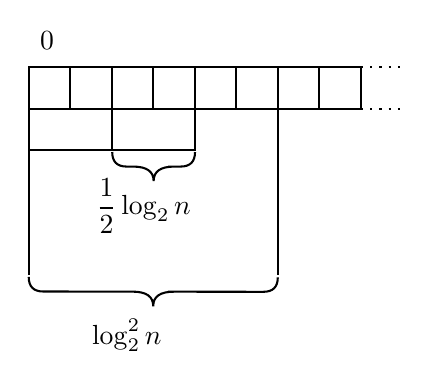
\begin{tikzpicture}[x=0.75pt,y=0.75pt,yscale=-1,xscale=1]
	\draw (150,231) .. controls (149.99,235.67) and (152.32,238) .. (156.99,238.01) -- (199.99,238.07) .. controls (206.66,238.08) and (209.99,240.41) .. (209.98,245.08) .. controls (209.99,240.41) and (213.32,238.09) .. (219.99,238.1)(216.99,238.09) -- (262.99,238.16) .. controls (267.66,238.17) and (269.99,235.84) .. (270,231.17);
	\draw (150,150) -- (150,230);
	\draw (270,150) -- (270,230);
	\draw (150,130) -- (170,130) -- (170,150) -- (150,150) -- cycle;
	\draw (170,130) -- (190,130) -- (190,150) -- (170,150) -- cycle;
	\draw (190,130) -- (210,130) -- (210,150) -- (190,150) -- cycle;
	\draw (210,130) -- (230,130) -- (230,150) -- (210,150) -- cycle;
	\draw (230,130) -- (250,130) -- (250,150) -- (230,150) -- cycle;
	\draw (250,130) -- (270,130) -- (270,150) -- (250,150) -- cycle;
	\draw (270,130) -- (290,130) -- (290,150) -- (270,150) -- cycle;
	\draw (290,130) -- (310,130) -- (310,150) -- (290,150) -- cycle;
	\draw (150,150) -- (190,150) -- (190,170) -- (150,170) -- cycle;
	\draw (190,150) -- (230,150) -- (230,170) -- (190,170) -- cycle;
	\draw (190.22,170.82) .. controls (190.22,175.49) and (192.55,177.82) .. (197.22,177.82) -- (200.17,177.82) .. controls (206.84,177.82) and (210.17,180.15) .. (210.17,184.82) .. controls (210.17,180.15) and (213.5,177.82) .. (220.17,177.82)(217.17,177.82) -- (223.11,177.82) .. controls (227.78,177.82) and (230.11,175.49) .. (230.11,170.82);
	\draw [dash pattern={on 0.84pt off 2.51pt}]  (310,130) -- (330,130);
	\draw [dash pattern={on 0.84pt off 2.51pt}]  (310,150) -- (330,150);

	\draw (179,250) node [anchor=north west][inner sep=0.75pt] [align=left] {$\displaystyle \log_2^2 n$};
	\draw (181,182) node [anchor=north west][inner sep=0.75pt] [align=left] {$\displaystyle \frac{1}{2} \log_2 n$};
	\draw (154,111.4) node [anchor=north west][inner sep=0.75pt] {$0$};
\end{tikzpicture}

	\caption{Divisione di $b$ in superblocchi e blocchi.}
	\label{fig:jrank}
\end{figure}

Si costruiscono quindi due vettori, $S$ e $B$. Per ogni superblocco $i$, $S_i$ contiene il rango del primo elemento di $b$ nel superblocco $i$. Per ogni blocco $j$, $B_j$ contiene la differenza tra il rango del primo elemento del blocco $j$ e il rango del primo elemento del relativo superblocco. Il rango di un elemento $p$ appartenente al superblocco $i$ e al blocco $j$ è quindi uguale a $S_i+B_j$ più il numero di bit a $1$ dall'inizio del blocco $j$ al bit $p$, ossia il rango di $p$ all'interno del sottovettore che coincide con il blocco $j$.

\begin{table}
	\centering
	\begin{tabular}{|c|c|c|c|c|c|c|}
		\hline
		\multirow{2}{*}{$0000$} & $p$        & $0$ & $1$ & $2$ & $3$ & $4$ \\ \cline{2-7}
		                        & $\rank(p)$ & $0$ & $0$ & $0$ & $0$ & $0$ \\ \hline
		\multirow{2}{*}{$0001$} & $p$        & $0$ & $1$ & $2$ & $3$ & $4$ \\ \cline{2-7}
		                        & $\rank(p)$ & $0$ & $0$ & $0$ & $0$ & $1$ \\ \hline
		$\cdots$                &            &     &     &     &     &     \\ \hline
		\multirow{2}{*}{$1111$} & $p$        & $0$ & $1$ & $2$ & $3$ & $4$ \\ \cline{2-7}
		                        & $\rank(p)$ & $0$ & $1$ & $2$ & $3$ & $4$ \\ \hline
	\end{tabular}
	\caption{Rango di ogni possibile blocco di lunghezza $4$.}
	\label{table:example_rank_block4}
\end{table}

I ranghi delle posizioni in un blocco sono salvati in un'apposita tabella, per evitare di doverli calcolare ogni volta. È quindi necessaria una tabella (simile a quanto mostrato in \cref{table:example_rank_block4}) che contiene il rango di ogni posizione, per ogni possibile tipo di blocco. I tipi di blocco possibili sono, in numero:
\begin{equation*}
	2^{\frac{1}{2}\log_2 n} = \left(2^{\log_2 n}\right)^{\frac{1}{2}} = \sqrt{n}
\end{equation*}

Il costo in bit di ogni tabella è
\begin{equation*}
	\underbrace{\frac{1}{2}\log_2 n}_\text{numero di elementi}\cdot \underbrace{\log_2\left(\frac{1}{2}\log_2 n\right)}_\text{costo dei valori di rango}
\end{equation*}
per un totale, per tutte le tabelle, di
\begin{equation*}
	\sqrt n\cdot\frac{1}{2}\log_2 n\cdot \log_2\left(\frac{1}{2}\log_2 n\right)
	\leq \sqrt n\cdot \frac{1}{2}\log_2 n\cdot \log_2(\log_2 n) = o(n) \text{ bit.}
\end{equation*}

Lo spazio occupato dal vettore $S$ è
\begin{equation*}
	\underbrace{\frac{n}{\log_2^2 n}}_\text{numero di superblocchi}\cdot\underbrace{\log_2 n}_\text{costo del singolo valore} = \frac{n}{\log_2 n} = o(n) \text{ bit}
\end{equation*}
Mentre quello occupato dal vettore $B$ è
\begin{equation*}
	\underbrace{\frac{n}{\frac{1}{2}\log_2 n}}_\text{numero di blocchi} \cdot\log_2(\log_2^2 n) =
	\frac{2n}{\log_2 n} 2 \log_2(\log_2 n) = o(n) \text{ bit}
\end{equation*}

% TODO migliorare figura (blocchi di 2 non sono molto rappresentativi)
\begin{figure}
	\centering
	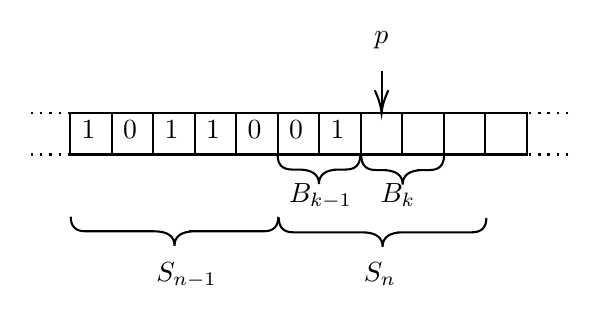
\begin{tikzpicture}[x=0.75pt,y=0.75pt,yscale=-1,xscale=1]
	\draw (100,100) -- (320,100) -- (320,120) -- (100,120) -- cycle;
	\draw (120,100) -- (120,120);
	\draw (140,100) -- (140,120);
	\draw (160,100) -- (160,120);
	\draw (180,100) -- (180,120);
	\draw (200,100) -- (200,120);
	\draw (220,100) -- (220,120);
	\draw (240,100) -- (240,120);
	\draw (260,100) -- (260,120);
	\draw (280,100) -- (280,120);
	\draw (300,100) -- (300,120);
	\draw (250,80) -- (250,98);
	\draw [shift={(250,100)}, rotate = 270] [color={rgb, 255:red, 0; green, 0; blue, 0 }  ][line width=0.75]    (10.93,-3.29) .. controls (6.95,-1.4) and (3.31,-0.3) .. (0,0) .. controls (3.31,0.3) and (6.95,1.4) .. (10.93,3.29);
	\draw (100.25,150) .. controls (100.25,154.67) and (102.58,157) .. (107.25,157) -- (140.25,157) .. controls (146.92,157) and (150.25,159.33) .. (150.25,164) .. controls (150.25,159.33) and (153.58,157) .. (160.25,157)(157.25,157) -- (193.25,157) .. controls (197.92,157) and (200.25,154.67) .. (200.25,150);
	\draw (200.5,150.5) .. controls (200.5,155.17) and (202.83,157.5) .. (207.5,157.5) -- (240.5,157.5) .. controls (247.17,157.5) and (250.5,159.83) .. (250.5,164.5) .. controls (250.5,159.83) and (253.83,157.5) .. (260.5,157.5)(257.5,157.5) -- (293.5,157.5) .. controls (298.17,157.5) and (300.5,155.17) .. (300.5,150.5);
	\draw [dash pattern={on 0.84pt off 2.51pt}] (100,100) -- (80,100);
	\draw [dash pattern={on 0.84pt off 2.51pt}] (100,120) -- (80,120);
	\draw [dash pattern={on 0.84pt off 2.51pt}] (340,120) -- (320,120);
	\draw [dash pattern={on 0.84pt off 2.51pt}] (340,100) -- (320,100);
	\draw (240.25,120.5) .. controls (240.25,125.17) and (242.58,127.5) .. (247.25,127.5) -- (250.17,127.5) .. controls (256.84,127.5) and (260.17,129.83) .. (260.17,134.5) .. controls (260.17,129.83) and (263.5,127.5) .. (270.17,127.5)(267.17,127.5) -- (273.08,127.5) .. controls (277.75,127.5) and (280.08,125.17) .. (280.08,120.5);
	\draw (199.92,120.25) .. controls (199.92,124.92) and (202.25,127.25) .. (206.92,127.25) -- (209.83,127.25) .. controls (216.5,127.25) and (219.83,129.58) .. (219.83,134.25) .. controls (219.83,129.58) and (223.16,127.25) .. (229.83,127.25)(226.83,127.25) -- (232.75,127.25) .. controls (237.42,127.25) and (239.75,124.92) .. (239.75,120.25);
	\draw (245,59.4) node [anchor=north west][inner sep=0.75pt] {$p$};
	\draw (104,102.4) node [anchor=north west][inner sep=0.75pt] {$1$};
	\draw (124,102.4) node [anchor=north west][inner sep=0.75pt] {$0$};
	\draw (144,102.4) node [anchor=north west][inner sep=0.75pt] {$1$};
	\draw (224,102.4) node [anchor=north west][inner sep=0.75pt] {$1$};
	\draw (164,102.4) node [anchor=north west][inner sep=0.75pt] {$1$};
	\draw (204,102.4) node [anchor=north west][inner sep=0.75pt] {$0$};
	\draw (240,170.4) node [anchor=north west][inner sep=0.75pt] {$S_{n}$};
	\draw (140,170.4) node [anchor=north west][inner sep=0.75pt] {$S_{n-1}$};
	\draw (248,132.4) node [anchor=north west][inner sep=0.75pt] {$B_{k}$};
	\draw (204,132.4) node [anchor=north west][inner sep=0.75pt] {$B_{k-1}$};
	\draw (184,102.4) node [anchor=north west][inner sep=0.75pt] {$0$};
\end{tikzpicture}

	\caption{Calcolo di $\rank(p)$.}
	\label{fig:example_rank_p}
\end{figure}

Un'implementazione della struttura succinta di Jacobson per il rango impiega un tempo costante per calcolare il rango di una posizione $p$, dovendo effettuare un accesso ai vettori $S$ e $B$ e uno alla tabella dei tipi di blocco. In effetti l'identificazione del tipo di blocco, stando al criterio di costo della macchina di Turing, è logaritmica in $n$, dovendo scansionare linearmente il blocco che contiene la posizione interessata. Tuttavia, adottando un criterio di costo simile alle macchine reali, questa scansione avviene in tempo costante, poiché un blocco è solitamente contenuto in una o due parole di memoria, recuperate in tempo costante.


\subsection{Struttura di Clarke per la selezione}
La struttura di Clarke per la selezione è succinta teoricamente, ma in pratica
è raramente utilizzata come descritta perché la sua implementazione è molto
complessa.
L'obiettivo è, dato un vettore $\mathbf{b}$ di valori binari fissato, calcolare
la funzione di selezione
$$
	\mathbf{select_b}(k) = \text{ posizione del } k-\text{esimo } 1
$$
La struttura di Clarke utilizza dei \textit{livelli}, simili a quelli utilizzati
dalla struttura di Jacobson.

\subsubsection{Primo livello}
Il primo livello della struttura di Clarke è un insieme
di valori che rappresentano le posizioni degli $1$ di ordinalità multipla di
$\log_2(n) \cdot \log_2(\log_2(n))$, ossia
$$
	P_i =  \mathbf{select_b}(i \cdot \log_2(n) \cdot \log_2(\log_2(n)))
$$
ossia la posizione del $(i \cdot \log_2(n) \cdot \log_2(\log_2(n)))$-esimo $1$.

\paragraph{Memoria}
La grandezza di questa famiglia, ossia il numero di $P_i$, dipende dal
numero di $i$ che ci sono in $\mathbf{b}$, ma nel caso peggiore, il vettore
è composto unicamente da $1$ e vi saranno $\frac{n}{\log_2(n) \cdot \log_2(\log_2(n))}$ membri.
Ad ognuno di essi va associato un elemento, il quale richiede $\log_2(n)$ bit;
in totale, questo livello occupa
$$
	\frac{n}{\log_2(n) \cdot \log_2(\log_2(n))} \cdot \log_2(n) = o(n) \text{ bit}
$$

\subsubsection{Secondo livello}
Per le posizioni che non sono multiple di $\log_2(n) \cdot \log_2(\log_2(n))$ si utilizza
un secondo livello, che è costruito differentemente in base ad un indice calcolato
per ogni $P_i$:

$$
	\forall i ~ r_i = P_{i + 1} - P_i
$$
che rappresenta la distanza fra l'$(i \cdot \log_2(n) \cdot \log_2(\log_2(n)))$-esimo $1$
e il $((i+1) \cdot \log_2(n) \cdot \log_2(\log_2(n)))$-esimo. Questo
valore, $r_i$, sarà esattamente uguale a $\log_2(n) \cdot \log_2(\log_2(n))$ se e solo se
tra $P_{i}$ e $P_{i+1}$ ci sono unicamente $1$, e sarà maggiore se invece le
due posizioni sono più lontane.
% @TODO: serve un esempio, non si capisce bene. 
I due casi che si considerano dipendono dal valore di $r_i$.

\paragraph{Caso sparso}
Se $r_i \geq (\log_2(n) \cdot \log_2(\log_2(n)))^2$, significa che in $\mathbf{b}$ ci
sono molti $0$ tra gli $1$ contenuti nelle posizioni tra $P_{i}$ e $P_{i+1}$; in questo caso
definiamo $S_i$ come la lista esplicita delle posizioni di tutti gli $1$
in $\mathbf{b}$ tra le due posizioni rappresentate come differenza tra $P_i$.

In questo caso, gli $S_i$ costruiti sono esattamente $\log_2(n)\cdot \log_2(\log_2(n))$,
in quanto stiamo contando gli $1$ in $\mathbf{b}$ tra il $(i \cdot \log_2(n) \cdot \log_2(\log_2(n))$-esimo
$1$ e il $((i+1) \cdot \log_2(n) \cdot \log_2(\log_2(n))$-esimo $1$, e ad ognuno
di essi si associa un numero che in grandezza è minore o uguale a
$\log_2(r_i)$, concludendo che per memorizzare un $S_i$ sono necessari
\begin{align*}
	\log_2(n)\cdot \log_2(\log_2(n)) \cdot \log_2(r_i) & = \frac{(\log_2(n)\cdot \log_2(\log_2(n)))^2}{\log_2(n)\cdot \log_2(\log_2(n))} \cdot \log_2(r_i) \\
	                                                   & \leq \frac{r_i}{\log_2(n)\cdot \log_2(\log_2(n))} \cdot \log_2(r_i)                               \\
	                                                   & \leq \frac{r_i}{\log_2(n)\cdot \log_2(\log_2(n))} \cdot \log_2(n)                                 \\
	                                                   & \leq \frac{r_i}{\log_2(\log_2(n))}                                                                \\
	                                                   & \leq \frac{n}{\log_2(\log_2(n))}   = o(n) \text{ bit}
\end{align*}

\paragraph{Caso denso}
Se $r_i \le (\log_2(n) \cdot \log_2(\log_2(n)))^2$, si memorizzano gli $1$
multipli di $\log_2(r_i)\log_2(\log_2(n))$, ossia partendo dalla posizione $P_i$ si salvano le
posizioni degli $j \cdot \log_2(r_i)\log_2(\log_2(n))$-esimi $1$ come differenze da $P_i$, ossia
$$
	S^i_j = \mathbf{select_b}(j \cdot \log_2(r_i)\log_2(\log_2(n))) - P_i
$$

In questo caso, gli $1$ memorizzati sono $\frac{\log_2(n)\cdot \log_2(\log_2(n))}{\log_2(r_i)\cdot \log_2(\log_2(n))}$.
Ad ognuno di questi si associa un valore in grandezza $\log_2(r_i)$, quindi lo spazio utilizzato
per memorizzare tutti i valori $S^i_j$ sono
$$
	\frac{\log_2(n)\cdot \log_2(\log_2(n))}{\log_2(r_i)\cdot \log_2(\log_2(n))} \log_2(r_i) =
	\frac{\log_2(n)\cdot \log_2(\log_2(n))}{\log_2(\log_2(n))} \leq \frac{r_i}{\log_2(\log_2(n))}
	\leq \frac{n}{\log_2(\log_2(n))} = o(n) \text{ bit}
$$


\subsubsection{Terzo livello}
Se nel secondo livello ci si trova nel caso denso, si utilizza un terzo livello.
Questo livello viene utilizzato esclusivamente per gli $1$ le cui posizioni non sono state
salvate nel secondo livello nel caso denso; pertanto, l'assunto è che
$$
	r_i < (\log_2(n) \log_2(\log_2(n)))^2
$$
Per ognuna di queste posizioni calcoliamo la differenza tra $S^i_j$:
$$
	\forall j ~~ \bar{r}^i_j = S^i_{j+1} - S^i_j
$$
Come nel caso precedente, abbiamo due possibilità in base al valore di $\bar{r}^i_j$, il quale
gode comunque della proprietà
$$
	\forall i, j ~~  \bar{r}^i_j \geq \log_2(r_i) \log_2(\log_2(n))
$$
\paragraph{Caso sparso}
Nel caso in cui $\bar{r}^i_j \geq \log_2(\bar{r}^i_j) \log_2(r_i) \log_2(\log_2(n))^2$,
si memorizzano esplicitamente tutte le posizioni degli $1$ tra $S^i_j$ e $S^i_{j+1}$
con dei valori $T^i_{j,k}$ come differenze tra $S^i_j$. In questo caso,
il consumo di memoria è
$$
	(\log_2(r_i)\cdot \log_2(\log_2(n)) \cdot \log_2(\bar{r}^i_j) \leq
	\frac{\log_2(r_i) \cdot \log_2(\log_2(n))^2 \log_2(\bar{r}^i_j)}{\log_2(\log_2(n))}
	\leq \frac{\bar{r}^i_j}{\log_2(\log_2(n))} = o(n) \text{ bit}
$$
\paragraph{Caso denso}
Nel caso in cui $\bar{r}^i_j \le \log_2(\bar{r}^i_j) \log_2(r_i) \log_2(\log_2(n))^2$,
significa che ci sono pochi $0$ tra $S^i_j$ e $S^i_{j+1}$ e
si utilizza il four-russians trick. Inizialmente osserviamo quanto segue.
\begin{oss}
	\begin{align*}
		\log_2(\bar{r}^i_j) \leq \log_2(r_i) & \leq \log_2(\log_2(n)\cdot \log_2(\log_2(n)))^2     \\
		                                     & = 2 \log_2(\log_2(n)) + 2 \log_2(\log_2(\log_2(n))) \\
		                                     & \leq 4 \log_2(\log_2(n))
	\end{align*}
\end{oss}
\begin{oss}
	$$
		\bar{r}^i_j < \log_2(\bar{r}^i_j) \cdot \log_2(r_i) \cdot (\log_2(\log_2(n))^2
		\leq 16(\log_2\log_2(n))^4
	$$
\end{oss}
Lo spazio necessario per utilizzare il four-russians trick è quanto segue.
Servono $2^{\bar{r}^i_j}$ enumerazioni di `sottovettori',
ossia la dimensione tra $S^i_j$ e $S^i_{j+1}$,
che è la parte che va memorizzata esplicitamente; per ognuna di queste
enumerazioni è necessario salvare la posizione di $\bar{r}^i_j$ $1$ utilizzando
memoria al massimo $\log_2(\bar{r}^i_j)$:
\begin{align*}
	2^{\bar{r}^i_j} \cdot \bar{r}^i_j \cdot \log_2(\bar{r}^i_j) & \leq
	2^{16(\log_2\log_2(n))^4} \cdot 16(\log_2\log_2(n))^4 \cdot \log_2(16(\log_2\log_2(n))^4)                                  \\
	                                                            & = 16(\log_2\log_2(n))^8 \log_2(16(\log_2\log_2(n))^4) = o(n)
\end{align*}


\subsubsection{Complessità totale in spazio}
In totale, per memorizzare $\mathbf{b}$ e i possibili tre livelli di struttura,
sono necessari $o(n)$ bit per il primo livello e, in base a come è fatto il secondo livello
$$
	\sum^{\frac{n}{\log_2(n)\cdot \log_2(\log_2(n))}} \frac{P_{i+1} - P_i}{\log_2(\log_2(n)}
	= \frac{P_n - P_0}{\log_2(\log_2(n))}
	\leq \frac{n}{\log_2(\log_2(n))} = o(n) \text{ bit}
$$
più $o(n)$ bit per il terzo livello. Quindi, la struttura di Clarke occupa
spazio $n + o(n)$ e ha tempo di accesso costante, pertanto è
una struttura \textbf{succinta}.

\begin{figure}
	\centering
	\tikzset{every picture/.style={line width=0.75pt}} %set default line width to 0.75pt        

	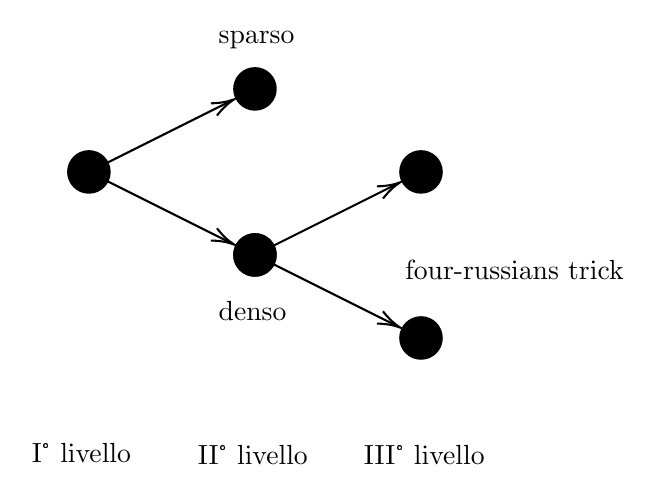
\begin{tikzpicture}[x=0.75pt,y=0.75pt,yscale=-1,xscale=1]
		%uncomment if require: \path (0,300); %set diagram left start at 0, and has height of 300

		%Shape: Circle [id:dp9914836432536758] 
		\draw  [fill={rgb, 255:red, 0; green, 0; blue, 0 }  ,fill opacity=1 ] (70,101) .. controls (70,95.48) and (74.48,91) .. (80,91) .. controls (85.52,91) and (90,95.48) .. (90,101) .. controls (90,106.52) and (85.52,111) .. (80,111) .. controls (74.48,111) and (70,106.52) .. (70,101) -- cycle ;
		%Shape: Circle [id:dp09703813871749656] 
		\draw  [fill={rgb, 255:red, 0; green, 0; blue, 0 }  ,fill opacity=1 ] (150,61) .. controls (150,55.48) and (154.48,51) .. (160,51) .. controls (165.52,51) and (170,55.48) .. (170,61) .. controls (170,66.52) and (165.52,71) .. (160,71) .. controls (154.48,71) and (150,66.52) .. (150,61) -- cycle ;
		%Straight Lines [id:da8346853138498954] 
		\draw    (80,101) -- (148.21,66.89) ;
		\draw [shift={(150,66)}, rotate = 153.43] [color={rgb, 255:red, 0; green, 0; blue, 0 }  ][line width=0.75]    (10.93,-3.29) .. controls (6.95,-1.4) and (3.31,-0.3) .. (0,0) .. controls (3.31,0.3) and (6.95,1.4) .. (10.93,3.29)   ;
		%Shape: Circle [id:dp4565729376211175] 
		\draw  [fill={rgb, 255:red, 0; green, 0; blue, 0 }  ,fill opacity=1 ] (150,141) .. controls (150,146.52) and (154.48,151) .. (160,151) .. controls (165.52,151) and (170,146.52) .. (170,141) .. controls (170,135.48) and (165.52,131) .. (160,131) .. controls (154.48,131) and (150,135.48) .. (150,141) -- cycle ;
		%Straight Lines [id:da8127484960209145] 
		\draw    (80,101) -- (148.21,135.11) ;
		\draw [shift={(150,136)}, rotate = 206.57] [color={rgb, 255:red, 0; green, 0; blue, 0 }  ][line width=0.75]    (10.93,-3.29) .. controls (6.95,-1.4) and (3.31,-0.3) .. (0,0) .. controls (3.31,0.3) and (6.95,1.4) .. (10.93,3.29)   ;
		%Shape: Circle [id:dp546530222511162] 
		\draw  [fill={rgb, 255:red, 0; green, 0; blue, 0 }  ,fill opacity=1 ] (150,141) .. controls (150,135.48) and (154.48,131) .. (160,131) .. controls (165.52,131) and (170,135.48) .. (170,141) .. controls (170,146.52) and (165.52,151) .. (160,151) .. controls (154.48,151) and (150,146.52) .. (150,141) -- cycle ;
		%Shape: Circle [id:dp1691093585413369] 
		\draw  [fill={rgb, 255:red, 0; green, 0; blue, 0 }  ,fill opacity=1 ] (230,101) .. controls (230,95.48) and (234.48,91) .. (240,91) .. controls (245.52,91) and (250,95.48) .. (250,101) .. controls (250,106.52) and (245.52,111) .. (240,111) .. controls (234.48,111) and (230,106.52) .. (230,101) -- cycle ;
		%Straight Lines [id:da17118221437478087] 
		\draw    (160,141) -- (228.21,106.89) ;
		\draw [shift={(230,106)}, rotate = 153.43] [color={rgb, 255:red, 0; green, 0; blue, 0 }  ][line width=0.75]    (10.93,-3.29) .. controls (6.95,-1.4) and (3.31,-0.3) .. (0,0) .. controls (3.31,0.3) and (6.95,1.4) .. (10.93,3.29)   ;
		%Shape: Circle [id:dp8870903616648642] 
		\draw  [fill={rgb, 255:red, 0; green, 0; blue, 0 }  ,fill opacity=1 ] (230,181) .. controls (230,186.52) and (234.48,191) .. (240,191) .. controls (245.52,191) and (250,186.52) .. (250,181) .. controls (250,175.48) and (245.52,171) .. (240,171) .. controls (234.48,171) and (230,175.48) .. (230,181) -- cycle ;
		%Straight Lines [id:da2110125336208042] 
		\draw    (160,141) -- (228.21,175.11) ;
		\draw [shift={(230,176)}, rotate = 206.57] [color={rgb, 255:red, 0; green, 0; blue, 0 }  ][line width=0.75]    (10.93,-3.29) .. controls (6.95,-1.4) and (3.31,-0.3) .. (0,0) .. controls (3.31,0.3) and (6.95,1.4) .. (10.93,3.29)   ;

		% Text Node
		\draw (51,230) node [anchor=north west][inner sep=0.75pt]   [align=left] {I° livello};
		% Text Node
		\draw (131,231) node [anchor=north west][inner sep=0.75pt]   [align=left] {II° livello};
		% Text Node
		\draw (211,231) node [anchor=north west][inner sep=0.75pt]   [align=left] {III° livello};
		% Text Node
		\draw (141,162) node [anchor=north west][inner sep=0.75pt]   [align=left] {denso};
		% Text Node
		\draw (141,32) node [anchor=north west][inner sep=0.75pt]   [align=left] {sparso};
		% Text Node
		\draw (231,142) node [anchor=north west][inner sep=0.75pt]   [align=left] {four-russians trick};
	\end{tikzpicture}
	\caption{Struttura di Clarke per la selezione.}
\end{figure}



\section{Alberi binari}
Un albero è un grafo non orientato, connesso e aciclico.
Un albero con radice è un albero in cui si elegge un vertice radice. I vertici adiacenti alla radice sono i suoi figli, che danno origine a sottoalberi. I vertici che danno origine a sottoalberi composti unicamente dalla radice sono detti foglie, o nodi esterni. I rimanenti nodi in un albero sono detti nodi interni.
Un albero binario è un albero radicato in cui ogni nodo interno ha due figli.
Equivalentemente si possono definire gli alberi binari induttivamente: un albero binario è una foglia $\emptyset$, oppure, se $L$ e $R$ sono alberi binari, è una coppia $(L,R)$ composta da una radice a cui sono connessi i sottoalberi $L$ e $R$.

% TODO: migliorare figura del passo induttivo: la radice dovrebbe essere adiacente alle radici dei sottoalberi
\begin{figure}
	\begin{subfigure}{0.45\textwidth}
	\begin{center}
		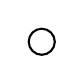
\begin{tikzpicture}
			\node [circle,draw]{};
		\end{tikzpicture}
	\end{center}
	\caption{Foglia}
\end{subfigure}
\begin{subfigure}{0.45\textwidth}
	\begin{center}
		\begin{tikzpicture}[subtree/.style={isosceles triangle,draw,shape border rotate=90}]
			\node[circle,draw] {}
			child { node[subtree] {$T_1$} }
			child { node[subtree] {$T_2$} };
		\end{tikzpicture}
	\end{center}
	\caption{Radice con due sottoalberi}
\end{subfigure}

	\caption{Definizione induttiva di albero binario.}
	\label{fig:btree_inductive}
\end{figure}

Un albero può essere \emph{ancillare}, cioè organizzare dati contenuti nei nodi interni o nelle foglie (tipicamente esclusivamente una delle due opzioni). Le strutture costruite per alberi privi di dati possono tipicamente essere generalizzate al caso di alberi ancillari.

Dato un albero binario, chiameremo $E$ l'insieme dei nodi esterni (foglie), $I$ l'insieme dei nodi interni e $n:=\card{I}$.
Definiamo inoltre le funzioni $\trext$ e $\trint$, definite rispettivamente come il numero di foglie e nodi interni di un dato albero binario.

\begin{theorem}\label{thm:btree_leaves}
	In un albero binario, il numero di foglie è uguale al numero di nodi interni più uno:
	\begin{equation*}
		\card{I}=\card{E}+1
	\end{equation*}
\end{theorem}
\begin{proof}
	Effettuando induzione strutturale sulla definizione di albero binario:
	\begin{itemize}
		\item $\trext(\emptyset)=1$, $\trint(\emptyset)=0$.
		\item siano $L, R$ due alberi binari. Vale
		      \begin{equation*}
			      \trext((L,R)) = \trext(L) + \trext(R) = \trint(L) + 1 + \trint(R) + 1 = \trint((L, R))  + 1
		      \end{equation*}
	\end{itemize}
\end{proof}

\begin{corollario}
	Ogni albero con $n$ nodi interni ha in totale $2n+1$ nodi.
\end{corollario}

\begin{theorem}
	Il numero di alberi binari con $n$ nodi interni è $C_n$, dove $C_n$ è l'$n$-esimo numero di Catalano:
	\begin{equation*}
		C_n := \frac{1}{n+1}\binom{2n}{n}
	\end{equation*}
\end{theorem}
\begin{corollario}
	\begin{equation*}
		\forall n \quad\log_2(C_n)=2n+O(\log_2(n))
	\end{equation*}
\end{corollario}
\begin{proof}
	Ricordando l'approssimazione di Stirling per il fattoriale:
	\begin{equation*}
		x! \sim \sqrt{2\pi x} \left(\frac{x}{e}\right)^x
	\end{equation*}
	si ha che
	\begin{align*}
		C_n = \frac{1}{n+1}\binom{2n}{n} & = \frac{1}{n+1}\cdot\frac{(2n)!}{n!(2n-n)!}                                                             \\
		                                 & = \frac{(2n)!}{(n+1)(n!)^2}                                                                             \\
		                                 & \sim \frac{\sqrt{4\pi n}\left(\frac{2n}{e}\right)^{2n}}{(n+1)\cdot 2\pi n\left(\frac{n}{e}\right)^{2n}} \\
		                                 & = \frac{1}{n+1}\cdot \frac{1}{\sqrt{\pi n}}\cdot 2^{2n}                                                 \\
		                                 & \approx \frac{4^n}{\sqrt{\pi n^3}}
	\end{align*}
	Da cui
	% TODO: spiegare
	\begin{equation*}
		\log_2 C_n = 2n-O(\log n) \text.
	\end{equation*}
\end{proof}
\begin{corollario}\label{corol:bitree:itlb}
	L'information theoretical lower bound in bit per gli alberi binari è
	\begin{equation*}
		Z_n = 2n-O(\log_2(n)) \text.
	\end{equation*}
\end{corollario}


\subsection{Una struttura succinta per alberi binari}
Per costruire una struttura succinta per gli alberi binari, definiamo tre operazioni fondamentali in cui possono consistere le query alla struttura dati: le operazioni $\trleft$ e $\trright$, che restituiscono rispettivamente il figlio sinistro e destro di un dato nodo, e l'operazione $\trparent$, che restituisce il genitore di un dato nodo.

Per rappresentare un albero binario con $n$ nodi interni, numeriamo i nodi da $0$ a $2n$ seguendo una visita in ampiezza, come rappresentato in \cref{fig:btree_rappr_num}.
Costruiamo quindi un vettore $v$ (\cref{fig:btree_rappr_vec}), di lunghezza $2n+1$ e tale che
\begin{equation*}
	\forall i\in\set{0,\dots,2n},\qquad v_i = \begin{cases}
		1 & \text{se il nodo $i$ appartiene a $I$} \\
		0 & \text{altrimenti}
	\end{cases}
\end{equation*}

\begin{figure}
	\centering
	\begin{subfigure}[t]{0.45\textwidth}
	\centering
	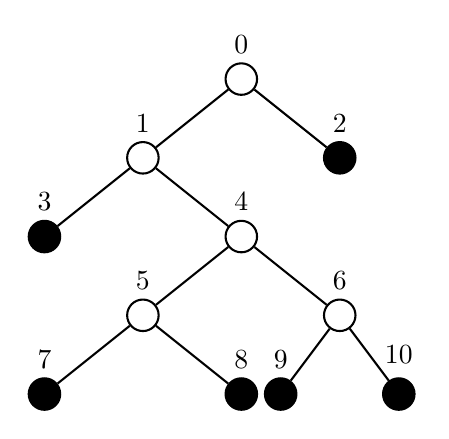
\begin{tikzpicture}[
			every node/.style={circle, draw, minimum size=4mm, inner sep=0.5mm},
			level distance=10mm,
			level 1/.style={sibling distance=25mm},
			level 2/.style={sibling distance=25mm}]
		\node [label=above:{0}]{}
		child {
		node [label=above:{1}] {}
		child {node[fill, label=above:{3}]{}}
		child {
		node[label=above:{4}]{}
		child {
		node [label=above:{5}]{}
		child {node[fill,label=above:{7}]{}}
		child {node[fill,label=above:{8}]{}}
		}
		child {
		node[label=above:{6}]  {}
		[level distance=10mm ,sibling distance=15mm]
		child {node[fill,label=above:{9}] {}}
		child {node[fill,label=above:{10}] {}}
		}
		}
		}
		child {node [fill, label=above:{2}]{}};
	\end{tikzpicture}

	\caption{Albero binario numerato.}
	\label{fig:btree_rappr_num}
\end{subfigure}
\begin{subfigure}[t]{0.45\textwidth}
	\centering
	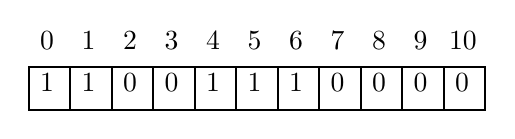
\begin{tikzpicture}[x=0.75pt,y=0.75pt,yscale=-1,xscale=1]
		\draw   (160,120) -- (180,120) -- (180,140.67) -- (160,140.67) -- cycle;
		\draw   (180,120) -- (200,120) -- (200,140.67) -- (180,140.67) -- cycle;
		\draw   (200,120) -- (220,120) -- (220,140.67) -- (200,140.67) -- cycle;
		\draw   (220,120) -- (240,120) -- (240,140.67) -- (220,140.67) -- cycle;
		\draw   (240,120) -- (260,120) -- (260,140.67) -- (240,140.67) -- cycle;
		\draw   (260,120) -- (280,120) -- (280,140.67) -- (260,140.67) -- cycle;
		\draw   (280,120) -- (300,120) -- (300,140.67) -- (280,140.67) -- cycle;
		\draw   (300,120) -- (320,120) -- (320,140.67) -- (300,140.67) -- cycle;
		\draw   (320,120) -- (340,120) -- (340,140.67) -- (320,140.67) -- cycle;
		\draw   (340,120) -- (360,120) -- (360,140.67) -- (340,140.67) -- cycle;
		\draw   (360,120) -- (380,120) -- (380,140.67) -- (360,140.67) -- cycle;
		\draw (164,101.4) node [anchor=north west][inner sep=0.75pt]    {$0$};
		\draw (184,101.4) node [anchor=north west][inner sep=0.75pt]    {$1$};
		\draw (204,101.4) node [anchor=north west][inner sep=0.75pt]    {$2$};
		\draw (224,101.4) node [anchor=north west][inner sep=0.75pt]    {$3$};
		\draw (244,101.4) node [anchor=north west][inner sep=0.75pt]    {$4$};
		\draw (264,101.4) node [anchor=north west][inner sep=0.75pt]    {$5$};
		\draw (284,101.4) node [anchor=north west][inner sep=0.75pt]    {$6$};
		\draw (304,101.4) node [anchor=north west][inner sep=0.75pt]    {$7$};
		\draw (324,101.4) node [anchor=north west][inner sep=0.75pt]    {$8$};
		\draw (344,101.46) node [anchor=north west][inner sep=0.75pt]    {$9$};
		\draw (361,101.4) node [anchor=north west][inner sep=0.75pt]    {$10$};
		\draw (164,121.4) node [anchor=north west][inner sep=0.75pt]    {$1$};
		\draw (184,121.4) node [anchor=north west][inner sep=0.75pt]    {$1$};
		\draw (204,121.4) node [anchor=north west][inner sep=0.75pt]    {$0$};
		\draw (224,121.4) node [anchor=north west][inner sep=0.75pt]    {$0$};
		\draw (244,121.4) node [anchor=north west][inner sep=0.75pt]    {$1$};
		\draw (264,121.4) node [anchor=north west][inner sep=0.75pt]    {$1$};
		\draw (284,121.4) node [anchor=north west][inner sep=0.75pt]    {$1$};
		\draw (304,121.4) node [anchor=north west][inner sep=0.75pt]    {$0$};
		\draw (324,121.4) node [anchor=north west][inner sep=0.75pt]    {$0$};
		\draw (344,121.46) node [anchor=north west][inner sep=0.75pt]    {$0$};
		\draw (364,121.4) node [anchor=north west][inner sep=0.75pt]    {$0$};
	\end{tikzpicture}
	\caption{Vettore associato all'albero.}
	\label{fig:btree_rappr_vec}
\end{subfigure}

	\caption{Un albero binario e il suo vettore associato.}
\end{figure}

Studiamo ora come produrre i risultati delle query di $\trleft$, $\trright$, e $\trparent$ a partire dal vettore $v$. Si consideri, all'interno di un albero $T$, una terna di nodi $p,q,q+1$, dove $p$ è il genitore e $q$ e $q+1$ i figli. Sia $T'$ il sottoalbero radicato nella stessa radice di $T$ contenente tutti i nodi di numero minore di $q$, come rappresentato in \cref{fig:btree_rappr_step}. Si tenga presente che alcuni nodi interni nell'albero $T$, in particolare quelli che seguono $p$, diventano foglie in $T'$.

Il numero di nodi interni minori di $p$, ossia il numero di nodi interni in $T'$, è uguale al rango di $p$ in $v$. Applicando il \cref{thm:btree_leaves}, calcoliamo che il numero complessivo di nodi minori di $q$, cioè il numero di nodi dell'albero $T'$, è
\begin{equation}\label{eq:btree:left_child}
	\trleft(p) = q = \trint(T')+\trext(T') = 2\cdot\trint(T')+1 = 2\cdot\rank(p)+1 \text.
\end{equation}
Mentre per il figlio destro vale, ovviamente
\begin{equation}\label{eq:btree:right_child}
	\trright(p) = q+1 = 2\cdot\rank(p)+1 \text.
\end{equation}

\begin{figure}
	\centering
	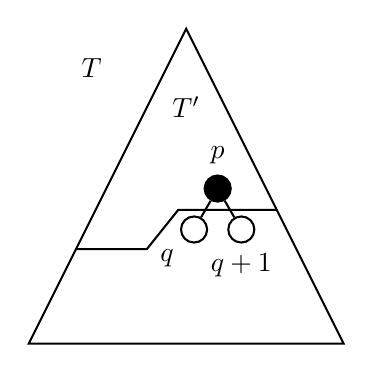
\begin{tikzpicture}[child/.style={draw,circle},father/.style={child,fill}]
  \draw (0,0) -- (4,0) -- (2,4) -- cycle;
  \draw (0.6,1.2) -- (1.5,1.2) -- (1.9,1.7) -- (3.15,1.7);
  \node (p) [father,label=above:{$p$}] at (2.4,1.97) {};
  \node (q) [child,label=below left:{$q$}] at (2.1,1.45) {};
  \node (qp) [child,label=below:{$q+1$}] at (2.7,1.45) {};
  \draw (p) -- (q);
  \draw (p) -- (qp);
  \node at (2,3) {$T'$};
  \node at (0.8,3.5) {$T$};
\end{tikzpicture}

	\caption{Sottoalbero $T'$ di $T$ utilizzato per calcolare $q$ e $q+1$.}
	\label{fig:btree_rappr_step}
\end{figure}

Per implementare l'operazione $\trparent$, si osservi che in virtù delle equazioni \ref{eq:btree:left_child} e \ref{eq:btree:right_child} vale
\begin{equation*}
	\begin{cases}
		\rank(p)=\dfrac{q}{2}-\dfrac12 & \quad\text{per $q$ dispari} \\[2ex]
		\rank(p)=\dfrac{q}{2}-1        & \quad\text{per $q$ pari}
	\end{cases}
\end{equation*}
da cui si ricava
\begin{equation*}
	\rank(p)=\floor{\frac x2-\frac 12}
\end{equation*}
e quindi, essendo $\select(\rank(p))=p$ poiché $v_p=1$:
\begin{equation*}
	p=\select(\rank(p))=\select\left(\floor{\frac x2-\frac 12}\right) \text.
\end{equation*}

È quindi possibile fare uso di una struttura per rappresentare il vettore $v$ che sia succinta rispetto all'information theoretical lower bound trovato al \cref{corol:bitree:itlb}:
\begin{align*}
	D_n & = 2n+1+o(n)    \\
	Z_n & = 2n-O(\log n)
\end{align*}



\section{Sequenze monotone}
Sia data una sequenza monotona di $n$ numeri naturali
\begin{equation*}
	x_0\leq x_1\leq \dots \leq x_{n-1}
\end{equation*}
Con un valore $u$, chiamato \emph{dimensione dell'universo}, tale che
\begin{equation*}
	\exists u ~ \forall i ~ x_i < u \text.
\end{equation*}

Dato un naturale $i<n$, si vuole ottenere l'elemento di indice $i$ della sequenza.


\subsection{La struttura di Elias-Fano}
Per evitare di usare un vettore di $n\cdot\log_2 u$ bit, viene definito un valore limite $l$:
\begin{equation*}
	l := \max\set{0,\floor{\log_2\left(\frac{u}{n}\right)}}\text.
\end{equation*}
La rappresentazione di Elias-Fano estrae da ogni intero $x_i$ la parte $l_i:=x_i\mod 2^l$, formata dai $l$ bit meno significativi. Per memorizzare le parti $l_i$ si fa uso di un vettore $L$ di $n$ elementi, ciascuno di $l$ bit.

Per le parti più significative, si calcolano i valori $u_i:=\floor{\frac{x_i}{2^l}}-\floor{\frac{x_{i-1}}{2^l}}$ (dove implicitamente $x_{-1}=0$), che vengono memorizzati in codifica unaria in una porzione di memoria $U$.

Poiché ci interessa il caso sparso, assumeremo $l\neq 0$, in quanto $l=0 \iff u<n$.


\subsubsection{Costo in spazio}
Il vettore $L$ ha costo, ovviamente, $l\cdot n$ bit.
Il numero di bit richiesti a memorizzare ciascun $u_i$ è uguale a $u_i+1$ ($u_i$ zeri e un $1$). In tutto
\begin{align*}
	\sum_{i=0}^{n-1}(u_i+1) & = \sum_{i=0}^{n-1}\left(\floor{\frac{x_i}{2^l}}-\floor{\frac{x_{i-1}}{2^l}}+1\right) \\
	                        & \leq n + \floor{\frac{x_{n-1}}{2^l}} \leq n + \frac{u}{2^l}                          \\[1ex]
	                        & \leq n+\frac{u}{2^{\floor{\log_2\frac{u}{n}}}}
\end{align*}
Se $u/n$ è una potenza di $2$, questo numero è uguale a $2n$, altrimenti è limitato da $3n$:
\begin{align*}
	 & \leq n+\frac{u}{2^{\log_2\frac{u}{n}-1}} \\[1ex]
	 & = n+\frac{2u}{u/n} = 3n \text.
\end{align*}
Considerando entrambe le parti, questa struttura occupa in spazio $l\cdot n$ bit per la parte inferiore e $2n$ o $3n$ bit per la parte superiore.
In totale, quindi, il costo è di $(l+2)n$ o $(l+3)n$ bit.
Ricordando l'ipotesi che $l=\floor{\log_2(u/n)}$, vale
\begin{equation*}
	\lceil \log_2(u/n) \rceil =
	\begin{cases}
		l & u/n \text{ è una potenza di } 2 \\
		l +1                                \\
	\end{cases}
\end{equation*}
Complessivamente, quindi, la struttura occupa un numero di bit di al più
\begin{equation*}
	D_n = 2n+n\ceil{\log_2\frac un} \text.
\end{equation*}


Per ricavare la parte più significativa di $x_i$ è necessario contare il numero di zeri fino all'$1$ di indice $i$ in $U$. Questo numero è uguale a $\select(i)-i$, quindi:
\begin{equation*}
	x_i=(\select(i)-i)2^l+l_i
\end{equation*}

Contando strutture succinte di rango e selezione rendere più efficiente il calcolo degli $x_i$, si ottiene un costo in spazio complessivo di
\begin{equation*}
	D_n = 2n+n\ceil{\log_2\frac un}+o(n) \text.
\end{equation*}


\subsection{Information theoretical lower bound}
Le possibili sequenze monotone di $n$ interi limitati da $u$ corrispondono ai possibili multisottoinsiemi dell'insieme $\set{0,\dots,u-1}$ di cardinalità $n$, nonché alle soluzioni dell'equazione
\begin{equation}\label{eq:seqmon}
	c_0+c_1+\dots+c_{u-1}
\end{equation}
dove $c_i$ è il numero di occorrenze dell'intero $i$ nella sequenza.

Per contare le possibili soluzioni si può utilizzare la tecnica \textit{stars and bars}, in
cui si utilizza una stringa costruita utilizzando $n$ stelline e $u-1$ barrette per rappresentare una soluzione all'equazione \ref{eq:seqmon}. Ad esempio:
\begin{equation*}
	| \starsymb || \starsymb \starsymb || \starsymb | \starsymb
\end{equation*}

Il valore complessivo della sequenza è $n$ e va distribuito in $u$ spazi, delineati dalle $u-1$ barrette.
L'interpretazione della stringa appena mostrata è $ c_0 = 0, c_1 = 1, c_2 = 0, c_3 = 2, c_4 = 0, c_5 = 1, c_6 = 1 $.
Il numero di soluzioni possibili è uguale al numero di stringhe costruite in questo modo, che equivale al numero di modi di scegliere $u-1$ posizioni in cui inserire barre in una stringa di $n+u-1$ simboli, ossia $\binom{n+u-1}{u - 1}$.

Facendo uso dell'approssimazione di Stirling per il coefficiente binomiale\footnote{$\log\binom AB \approx B\log\frac AB+(A-B)\log\frac{A}{A-B}$. In questo caso $A:=u+n-1$ e $B:=n$, quindi per $n\ll u$ il secondo addendo si annulla.}:
\begin{align*}
	Z_n & = \log_2\binom{n+u-1}{u - 1} = \log_2\binom{n+u-1}{n}              \\
	    & \approx n\log_2\frac{u+n-1}{n} =                                   \\
	    & = n\log_2\left(\frac un\left(1+\frac nu - \frac 1u\right)\right) = \\
	    & = n\log_2\frac un + n\log_2\left(1+\frac nu-\frac 1u\right)        \\
	    & \sim n\log_2\frac un + \frac{n^2}{u} \approx n\log_2\frac un
\end{align*}

Quindi la struttura è implicita:
\begin{equation*}
	D_n = 2n+n\ceil{\log_2\frac un}+o(n) = O(Z_n)
\end{equation*}



\section{Struttura per parentesi ben formate}
\subsection{Linguaggi di Dyck}
Un linguaggio di Dyck $L$ è un linguaggio sull'alfabeto $D=\{(,)\}$ tale che $L \subseteq D^*$
e una stringa $w \in D^*$ appartiene a $L$ se e solo se
\begin{enumerate}
	\item $|w|_{(} = |w|_{)}$; e
	\item $\forall w_1, w_2 \text{ tali che } w = w_1w_2 \implies|w_1|_{(} \geq |w_2|_{)}$
\end{enumerate}
Un modo interessante per studiare una parola $w$ di Dyck è studiarne la
\textit{funzione di eccesso}, definita
$$
	E_w(i) = |\{j | j \le i ~ w_j = ( ~\}| - |\{j | j \leq i ~ w_j = ) ~\}|
$$
\begin{figure}[h]
	\centering
	\begin{tikzpicture}
		\draw[->] (-1, 0) -- (8.50, 0) node[right] {$x$};
		\draw[->] (-1, 0) -- (-1, 4) node[above] {$y$};

		\draw (0,0) node[circle,fill,inner sep=1pt, label=above:{(}] {} -- (1,1) node[circle,fill,inner sep=1pt]{};
		\draw (1,1) node[circle,fill,inner sep=1pt, label=above:{(}] {} -- (2,1) node[circle,fill,inner sep=1pt]{};
		\draw (2,1) node[circle,fill,inner sep=1pt, label=above:{)}] {} -- (3,1) node[circle,fill,inner sep=1pt]{};
		\draw (3,1) node[circle,fill,inner sep=1pt, label=above:{(}] {} -- (4,2) node[circle,fill,inner sep=1pt]{};
		\draw (4,2) node[circle,fill,inner sep=1pt, label=above:{(}] {} -- (5,2) node[circle,fill,inner sep=1pt]{};
		\draw (5,2) node[circle,fill,inner sep=1pt, label=above:{)}] {} -- (6,1) node[circle,fill,inner sep=1pt]{};
		\draw (6,1) node[circle,fill,inner sep=1pt, label=above:{)}] {} -- (7,0) node[circle,fill,inner sep=1pt, label=above:{)}]{};
	\end{tikzpicture}
	\caption{Funzione di eccesso per la parola $(()(()))$.}
	\label{fig:func_excess}
\end{figure}

Questa funzione parte da $0$, può tornare a $0$ e, se la parola è effettivamente nel
linguaggio, termina a $0$. Ci sono due tipi di stringhe di Dyck: quelle per cui
la funzione non raggiunge nessuno $0$ tranne quello iniziale e quello finale,
chiamate \textit{fortemente bilanciate}, e quelle per cui questa funzione raggiunge
uno $0$ diverso da quello iniziale e quello finale, quindi $w = w_1w_2$ è
\textit{debolmente bilanciata} e tale per cui almeno uno tra $w_1$ e $w_2$ è
fortemente bilanciata.

Ci sono molti motivi per cui le sequenze di parentesi sono interessanti. In particolare,
le espressioni ben parentesizzate sono in biiezione sia con le foreste di alberi binari che con gli
alberi non binari. In qualche modo, esattamente come abbiamo visto una rappresentazione
per gli alberi binari in precedenza, ora stiamo analizzando una struttura per alberi
generali. Le sequenze di parentesi aperte e chiuse le penseremo come stringhe di bit, cioè
una stringa
$$
	(()(()())(()))
$$
è rappresentata come una stringa
$$
	11011010011000
$$
la cui funzione di eccesso è rappresentata in \cref{fig:func_excess_example}.

\begin{figure}[h]
	\centering
	\begin{tikzpicture}
		\draw[->] (-1, 0) -- (14.5, 0) node[right] {$x$};
		\draw[->] (-1, 0) -- (-1, 4) node[above] {$y$};

		\draw (0,0) node[label=above:{(}]	{} -- 	(1,1) node[circle,fill,inner sep=1pt]{};
		\draw (1,1) node[label=above:{(}] 	{} -- 	(2,1) node[circle,fill,inner sep=1pt]{};
		\draw (2,1) node[label=above:{)}] 	{} -- 	(3,1) node[circle,fill,inner sep=1pt]{};
		\draw (3,1) node[label=above:{(}] 	{} -- 	(4,2) node[circle,fill,inner sep=1pt]{};
		\draw (4,2) node[label=above:{(}] 	{} -- 	(5,2) node[circle,fill,inner sep=1pt]{};
		\draw (5,2) node[label=above:{)}] 	{} -- 	(6,2) node[circle,fill,inner sep=1pt]{};
		\draw (6,2) node[label=above:{(}] 	{} -- 	(7,2) node[circle,fill,inner sep=1pt]{};
		\draw (7,2) node[label=above:{)}] 	{} -- 	(8,1) node[circle,fill,inner sep=1pt]{};
		\draw (8,1) node[label=above:{)}] 	{} -- 	(9,1) node[circle,fill,inner sep=1pt]{};
		\draw (9,1) node[label=above:{(}] 	{} -- 	(10,2) node[circle,fill,inner sep=1pt]{};
		\draw (10,2) node[label=above:{(}]  	{} -- 	(11,2) node[circle,fill,inner sep=1pt]{};
		\draw (11,2) node[label=above:{)}]  	{} -- 	(12,1) node[circle,fill,inner sep=1pt]{};
		\draw (12,1) node[label=above:{)}]  	{} -- 	(13,0) node[circle,fill,inner sep=1pt,label=above:{)}]{};
	\end{tikzpicture}
	\caption{Funzione di eccesso per la parola $(()(()())(()))$.}
	\label{fig:func_excess_example}
\end{figure}

\subsection{L'ADT stringa bilanciata}
L'ADT che vogliamo descrivere per le stringhe di parentesi ben bilanciate ha le primitive
$$
	\forall p \in \mathbb{N} ~~ \mathbf{find\_open}(p) = \text{parentesi aperta corrispondente alla chiusa in posizione } p
$$
$$
	\forall p \in \mathbb{N} ~~ \mathbf{find\_close}(p) = \text{parentesi chiusa corrispondente all'aperta in posizione } p
$$
$$
	\forall p \in \mathbb{N} ~~ \mathbf{enclose}(p) = \text{prima parentesi aperta che racchiude la parentesi in posizione } p
$$

Pensando ad una soluzione banale, una $\mathbf{find\_open}$ in una qualche posizione si può
calcolare innanzitutto realizzando che la parentesi aperta corrispondente ad una
parentesi chiusa è sicuramente prima della chiusa stessa; basta quindi cercare all'indietro fermandosi
alla prima parentesi aperta che ha la stessa funzione di eccesso. Analogamente si fa per $\mathbf{find\_close}$.
La cosa più semplice, quindi, sarebbe calcolare anticipatamente la funzione di eccesso e usarla
facendo ricerche lineari, utilizzando uno spazio $n \log_2(n)$.
Faremo meglio creando una struttura compatta con tempo di interrogazione logaritmico.

\subsubsection{Rappresentazione}
La prima operazione sulle parentesi da eseguire nella costruzione della struttura è dividere, nuovamente,
la parola in blocchi di lunghezza $l$, creando $k = \lceil n/l \rceil$ blocchi. In ogni blocco
ci sono parentesi chiuse e aperte e, in alcuni casi, le parentesi hanno la loro corrispondente
dentro il blocco stesso: in questa situazione, definiamo la parentesi \textit{vicina}, mentre
tutte le altri sono definite \textit{lontane}; in generale, tutte le parentesi aperte lontane
si chiuderanno in un qualche blocco successivo.

In ogni blocco ci sono alcune parentesi vicine e varie parentesi lontane. Può succedere
che una o più parentesi lontane si chiudano nello stesso blocco: definiamo \textit{pioniera}
la lontana aperta (benché si possa fare lo stesso ragionamento, a specchio, per le chiuse)
che è la prima del blocco al quale appartiene a chiudersi in un qualsiasi altro blocco successivo.
Un esempio di queste divisioni è in \cref{fig:paren_blocks}, dove le parentesi gialle sono le vicine,
quelle blu sono lontane e quelle rosse sono pioniere.

\begin{figure}[h]

	\centering

	\tikzset{every picture/.style={line width=0.75pt}} %set default line width to 0.75pt        

	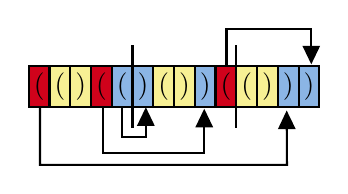
\begin{tikzpicture}[x=0.75pt,y=0.75pt,yscale=-1,xscale=1]
		%uncomment if require: \path (0,300); %set diagram left start at 0, and has height of 300

		%Shape: Rectangle [id:dp12028039856705786] 
		\draw  [fill={rgb, 255:red, 208; green, 2; blue, 27 }  ,fill opacity=1 ] (160,170) -- (170,170) -- (170,190) -- (160,190) -- cycle ;

		%Shape: Rectangle [id:dp6017350169887977] 
		\draw  [fill={rgb, 255:red, 247; green, 240; blue, 148 }  ,fill opacity=1 ] (170,170) -- (180,170) -- (180,190) -- (170,190) -- cycle ;

		%Shape: Rectangle [id:dp1862637830525412] 
		\draw  [fill={rgb, 255:red, 247; green, 240; blue, 148 }  ,fill opacity=1 ] (180,170) -- (190,170) -- (190,190) -- (180,190) -- cycle ;

		%Shape: Rectangle [id:dp7375538410378665] 
		\draw  [fill={rgb, 255:red, 208; green, 2; blue, 27 }  ,fill opacity=1 ] (190,170) -- (200,170) -- (200,190) -- (190,190) -- cycle ;

		%Shape: Rectangle [id:dp42832713437851455] 
		\draw  [fill={rgb, 255:red, 139; green, 181; blue, 229 }  ,fill opacity=1 ] (200,170) -- (210,170) -- (210,190) -- (200,190) -- cycle ;

		%Shape: Rectangle [id:dp3771120606312378] 
		\draw  [fill={rgb, 255:red, 139; green, 181; blue, 229 }  ,fill opacity=1 ] (210,170) -- (220,170) -- (220,190) -- (210,190) -- cycle ;

		%Shape: Rectangle [id:dp19892421904849122] 
		\draw  [fill={rgb, 255:red, 247; green, 240; blue, 148 }  ,fill opacity=1 ] (220,170) -- (230,170) -- (230,190) -- (220,190) -- cycle ;

		%Shape: Rectangle [id:dp0006276055923941648] 
		\draw  [fill={rgb, 255:red, 247; green, 240; blue, 148 }  ,fill opacity=1 ] (230,170) -- (240,170) -- (240,190) -- (230,190) -- cycle ;

		%Shape: Rectangle [id:dp16538357452442487] 
		\draw  [fill={rgb, 255:red, 139; green, 181; blue, 229 }  ,fill opacity=1 ] (240,170) -- (250,170) -- (250,190) -- (240,190) -- cycle ;

		%Shape: Rectangle [id:dp06112380309966958] 
		\draw  [fill={rgb, 255:red, 208; green, 2; blue, 27 }  ,fill opacity=1 ] (250,170) -- (260,170) -- (260,190) -- (250,190) -- cycle ;

		%Shape: Rectangle [id:dp06951356935410424] 
		\draw  [fill={rgb, 255:red, 247; green, 240; blue, 148 }  ,fill opacity=1 ] (260,170) -- (270,170) -- (270,190) -- (260,190) -- cycle ;

		%Shape: Rectangle [id:dp885838800749071] 
		\draw  [fill={rgb, 255:red, 247; green, 240; blue, 148 }  ,fill opacity=1 ] (270,170) -- (280,170) -- (280,190) -- (270,190) -- cycle ;

		%Shape: Rectangle [id:dp37752499309076915] 
		\draw  [fill={rgb, 255:red, 139; green, 181; blue, 229 }  ,fill opacity=1 ] (280,170) -- (290,170) -- (290,190) -- (280,190) -- cycle ;

		%Shape: Rectangle [id:dp7109616333523956] 
		\draw  [fill={rgb, 255:red, 139; green, 181; blue, 229 }  ,fill opacity=1 ] (290,170) -- (300,170) -- (300,190) -- (290,190) -- cycle ;

		%Straight Lines [id:da856450147041028] 
		\draw    (210,160) -- (210,200) ;
		%Straight Lines [id:da0823905364290688] 
		\draw    (260,160) -- (260,200) ;
		%Straight Lines [id:da8657156752341498] 
		\draw    (205.14,190.29) -- (205.14,204.36) -- (216.43,204.36) -- (216.43,192.93) ;
		\draw [shift={(216.43,189.93)}, rotate = 90] [fill={rgb, 255:red, 0; green, 0; blue, 0 }  ][line width=0.08]  [draw opacity=0] (8.93,-4.29) -- (0,0) -- (8.93,4.29) -- cycle    ;
		%Straight Lines [id:da4613663625082196] 
		\draw    (195.57,189.79) -- (195.57,212.07) -- (244.57,212.07) -- (244.57,193.64) ;
		\draw [shift={(244.57,190.64)}, rotate = 90] [fill={rgb, 255:red, 0; green, 0; blue, 0 }  ][line width=0.08]  [draw opacity=0] (8.93,-4.29) -- (0,0) -- (8.93,4.29) -- cycle    ;
		%Straight Lines [id:da9063548393327128] 
		\draw    (165.43,190.21) -- (165.43,217.64) -- (284.43,217.64) -- (284.3,194.5) ;
		\draw [shift={(284.29,191.5)}, rotate = 89.69] [fill={rgb, 255:red, 0; green, 0; blue, 0 }  ][line width=0.08]  [draw opacity=0] (8.93,-4.29) -- (0,0) -- (8.93,4.29) -- cycle    ;
		%Straight Lines [id:da09579212789908009] 
		\draw    (255.29,170.21) -- (255.29,152.07) -- (296.14,152.07) -- (296.14,166.21) ;
		\draw [shift={(296.14,169.21)}, rotate = 270] [fill={rgb, 255:red, 0; green, 0; blue, 0 }  ][line width=0.08]  [draw opacity=0] (8.93,-4.29) -- (0,0) -- (8.93,4.29) -- cycle    ;

		% Text Node
		\draw (161,172) node [anchor=north west][inner sep=0.75pt]   [align=left] {(};
		% Text Node
		\draw (171,172) node [anchor=north west][inner sep=0.75pt]   [align=left] {(};
		% Text Node
		\draw (181,172) node [anchor=north west][inner sep=0.75pt]   [align=left] {)};
		% Text Node
		\draw (211,172) node [anchor=north west][inner sep=0.75pt]   [align=left] {)};
		% Text Node
		\draw (201,172) node [anchor=north west][inner sep=0.75pt]   [align=left] {(};
		% Text Node
		\draw (191,172) node [anchor=north west][inner sep=0.75pt]   [align=left] {(};
		% Text Node
		\draw (271,172) node [anchor=north west][inner sep=0.75pt]   [align=left] {)};
		% Text Node
		\draw (261,172) node [anchor=north west][inner sep=0.75pt]   [align=left] {(};
		% Text Node
		\draw (251,172) node [anchor=north west][inner sep=0.75pt]   [align=left] {(};
		% Text Node
		\draw (241,172) node [anchor=north west][inner sep=0.75pt]   [align=left] {)};
		% Text Node
		\draw (231,172) node [anchor=north west][inner sep=0.75pt]   [align=left] {)};
		% Text Node
		\draw (221,172) node [anchor=north west][inner sep=0.75pt]   [align=left] {(};
		% Text Node
		\draw (291,172) node [anchor=north west][inner sep=0.75pt]   [align=left] {)};
		% Text Node
		\draw (281,172) node [anchor=north west][inner sep=0.75pt]   [align=left] {)};
	\end{tikzpicture}

	\caption{Divisione in blocchi di una stringa parentesizzata.}
	\label{fig:paren_blocks}
\end{figure}

Assumiamo che $w$ sia la parola da rappresentare e assumiamo che $|w| = n$.
Per rappresentare la parola memorizziamo, oltre a $w$ stessa, un vettore $\mathbf{p}$ di $n$ bit
con $1$ nelle posizioni delle pioniere; il vettore $\mathbf{E}$, che per ogni blocco $i$
da l'eccesso all'inizio del blocco e ha un elemento per ogni blocco; il vettore $\mathbf{M}$, che per ogni
blocco $i$ mantiene la posizione della parentesi corrispondente all'$i$-esima pioniera e, infine, il vettore
$\mathbf{O}$ che per ogni blocco $i$ mantiene la posizione della prima aperta a sinistra dell'inizio del blocco
avente eccesso $x-1$, dove $x$ è il minimo eccesso del blocco. Per la rappresentazione, definiamo $l = \log_2(n)$.
\begin{theorem}
	Se ci sono $k$ blocchi, vi sono al massimo $2^k - 3$ coppie di pionieri.
\end{theorem}
\begin{proof}
	Costruiamo un grafo $G = (V, E)$ dove $V$ sono i blocchi ed esiste un lato tra un blocco $x$ e $y$ se
	e solo se $x$ contiene una pioniera cha ha in $y$ la sua corrispondente.
	Dimostriamo per induzione su $k$: vi sono due casi.
	\begin{itemize}
		\item se l'insieme di blocchi è separabile, ossia esiste una posizione nella parola sulla quale
		      ``non passano archi'', la parola è debolmente bilanciate ed è scomponibile in due diverse
		      parole ben formate. Allora, per ipotesi induttiva, il numero di pioniere nella prima
		      parte è al più $2p - 3$ e il numero di pioniere nella seconda parte è al più $2(k - p + 1) - 3$;
		      allora il numero di pioniere è al più
		      $$
			      2p - 3 + 2 k - 2p + 2 - 3 = 2k - 4 \leq 2k - 3
		      $$
		\item se l'insieme di blocchi non è separabile, ossia la parola è fortemente
		      bilanciate e non è scomponibile in due parole diverse, si prende la
		      prima coppia di parentesi lontane che si trova in $w$ e si rimuove. La parola risultante,
		      che chiamiamo $w'$, gode della proprietà che si vuole dimostrare. Il numero
		      di pioniere in $w$ è quindi al più la somma delle pioniere in $w'$ e la pioniera rimossa
		      $$
			      2k - 4  + 1 = 2k - 3
		      $$

	\end{itemize}
\end{proof}

\begin{figure}[h]
	\centering
	\begin{subfigure}{0.45\textwidth}
		\centering
		\tikzset{every picture/.style={line width=0.75pt}} %set default line width to 0.75pt        
		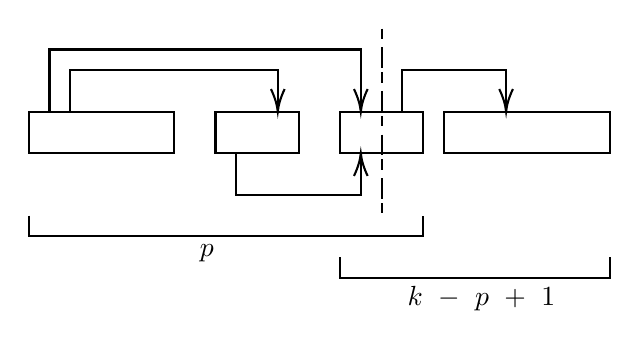
\begin{tikzpicture}[x=0.75pt,y=0.75pt,yscale=-1,xscale=1]
			%uncomment if require: \path (0,300); %set diagram left start at 0, and has height of 300

			%Shape: Rectangle [id:dp5751448069992374] 
			\draw   (100,130) -- (170,130) -- (170,150) -- (100,150) -- cycle ;
			%Shape: Rectangle [id:dp8956649728081978] 
			\draw   (190,130) -- (230,130) -- (230,150) -- (190,150) -- cycle ;
			%Shape: Rectangle [id:dp8836798951210239] 
			\draw   (250,130) -- (290,130) -- (290,150) -- (250,150) -- cycle ;
			%Shape: Rectangle [id:dp07169651712981018] 
			\draw   (300,130) -- (380,130) -- (380,150) -- (300,150) -- cycle ;
			%Straight Lines [id:da8396678932783305] 
			\draw    (110,130) -- (110,100) -- (260,100) -- (260,128) ;
			\draw [shift={(260,130)}, rotate = 270] [color={rgb, 255:red, 0; green, 0; blue, 0 }  ][line width=0.75]    (10.93,-3.29) .. controls (6.95,-1.4) and (3.31,-0.3) .. (0,0) .. controls (3.31,0.3) and (6.95,1.4) .. (10.93,3.29)   ;
			%Straight Lines [id:da8376287767119306] 
			\draw    (120,130) -- (120,110) -- (220,110) -- (220,128) ;
			\draw [shift={(220,130)}, rotate = 270] [color={rgb, 255:red, 0; green, 0; blue, 0 }  ][line width=0.75]    (10.93,-3.29) .. controls (6.95,-1.4) and (3.31,-0.3) .. (0,0) .. controls (3.31,0.3) and (6.95,1.4) .. (10.93,3.29)   ;
			%Straight Lines [id:da7343053938900628] 
			\draw    (200,150) -- (200,170) -- (260,170) -- (260,152) ;
			\draw [shift={(260,150)}, rotate = 90] [color={rgb, 255:red, 0; green, 0; blue, 0 }  ][line width=0.75]    (10.93,-3.29) .. controls (6.95,-1.4) and (3.31,-0.3) .. (0,0) .. controls (3.31,0.3) and (6.95,1.4) .. (10.93,3.29)   ;
			%Straight Lines [id:da02843704523195245] 
			\draw    (280,130) -- (280,110) -- (330,110) -- (330,128) ;
			\draw [shift={(330,130)}, rotate = 270] [color={rgb, 255:red, 0; green, 0; blue, 0 }  ][line width=0.75]    (10.93,-3.29) .. controls (6.95,-1.4) and (3.31,-0.3) .. (0,0) .. controls (3.31,0.3) and (6.95,1.4) .. (10.93,3.29)   ;
			%Straight Lines [id:da4532725638041315] 
			\draw  [dash pattern={on 3.75pt off 3pt on 7.5pt off 1.5pt}]  (270,90) -- (270,180) ;
			%Straight Lines [id:da17944476616348748] 
			\draw    (100,180) -- (100,190) -- (290,190) -- (290,180) ;
			%Straight Lines [id:da1753890360224526] 
			\draw    (250,200) -- (250,210) -- (380,210) -- (380,200) ;

			% Text Node
			\draw (181,192.4) node [anchor=north west][inner sep=0.75pt]    {$p$};
			% Text Node
			\draw (281,212.4) node [anchor=north west][inner sep=0.75pt]    {$k\ -\ p\ +\ 1$};
		\end{tikzpicture}
		\subcaption{Caso $1$.}
	\end{subfigure}
	\hfill
	\begin{subfigure}{0.45\textwidth}

		\tikzset{
			pattern size/.store in=\mcSize,
			pattern size = 5pt,
			pattern thickness/.store in=\mcThickness,
			pattern thickness = 0.3pt,
			pattern radius/.store in=\mcRadius,
			pattern radius = 1pt}
		\makeatletter
		\pgfutil@ifundefined{pgf@pattern@name@_y43ms7xnt}{
			\pgfdeclarepatternformonly[\mcThickness,\mcSize]{_y43ms7xnt}
			{\pgfqpoint{0pt}{-\mcThickness}}
			{\pgfpoint{\mcSize}{\mcSize}}
			{\pgfpoint{\mcSize}{\mcSize}}
			{
				\pgfsetcolor{\tikz@pattern@color}
				\pgfsetlinewidth{\mcThickness}
				\pgfpathmoveto{\pgfqpoint{0pt}{\mcSize}}
				\pgfpathlineto{\pgfpoint{\mcSize+\mcThickness}{-\mcThickness}}
				\pgfusepath{stroke}
			}}
		\makeatother

		% Pattern Info

		\tikzset{
			pattern size/.store in=\mcSize,
			pattern size = 5pt,
			pattern thickness/.store in=\mcThickness,
			pattern thickness = 0.3pt,
			pattern radius/.store in=\mcRadius,
			pattern radius = 1pt}
		\makeatletter
		\pgfutil@ifundefined{pgf@pattern@name@_mifsyi5bu}{
			\pgfdeclarepatternformonly[\mcThickness,\mcSize]{_mifsyi5bu}
			{\pgfqpoint{0pt}{0pt}}
			{\pgfpoint{\mcSize+\mcThickness}{\mcSize+\mcThickness}}
			{\pgfpoint{\mcSize}{\mcSize}}
			{
				\pgfsetcolor{\tikz@pattern@color}
				\pgfsetlinewidth{\mcThickness}
				\pgfpathmoveto{\pgfqpoint{0pt}{0pt}}
				\pgfpathlineto{\pgfpoint{\mcSize+\mcThickness}{\mcSize+\mcThickness}}
				\pgfusepath{stroke}
			}}
		\makeatother
		\tikzset{every picture/.style={line width=0.75pt}} %set default line width to 0.75pt        

		\begin{tikzpicture}[x=0.75pt,y=0.75pt,yscale=-1,xscale=1]
			%uncomment if require: \path (0,300); %set diagram left start at 0, and has height of 300

			%Shape: Rectangle [id:dp5339690558371227] 
			\draw   (120,150) -- (190,150) -- (190,170) -- (120,170) -- cycle ;
			%Straight Lines [id:da850734740747954] 
			\draw    (140,150) -- (140,120) -- (280,120) -- (280,148) ;
			\draw [shift={(280,150)}, rotate = 270] [color={rgb, 255:red, 0; green, 0; blue, 0 }  ][line width=0.75]    (10.93,-3.29) .. controls (6.95,-1.4) and (3.31,-0.3) .. (0,0) .. controls (3.31,0.3) and (6.95,1.4) .. (10.93,3.29)   ;
			%Straight Lines [id:da9735874841202442] 
			\draw    (150,150) -- (150,130) -- (240,130) -- (240,148) ;
			\draw [shift={(240,150)}, rotate = 270] [color={rgb, 255:red, 0; green, 0; blue, 0 }  ][line width=0.75]    (10.93,-3.29) .. controls (6.95,-1.4) and (3.31,-0.3) .. (0,0) .. controls (3.31,0.3) and (6.95,1.4) .. (10.93,3.29)   ;
			%Straight Lines [id:da863983070784418] 
			\draw    (220,170) -- (220,190) -- (280,190) -- (280,172) ;
			\draw [shift={(280,170)}, rotate = 90] [color={rgb, 255:red, 0; green, 0; blue, 0 }  ][line width=0.75]    (10.93,-3.29) .. controls (6.95,-1.4) and (3.31,-0.3) .. (0,0) .. controls (3.31,0.3) and (6.95,1.4) .. (10.93,3.29)   ;
			%Straight Lines [id:da6442133803721162] 
			\draw    (300,150) -- (300,130) -- (350,130) -- (350,148) ;
			\draw [shift={(350,150)}, rotate = 270] [color={rgb, 255:red, 0; green, 0; blue, 0 }  ][line width=0.75]    (10.93,-3.29) .. controls (6.95,-1.4) and (3.31,-0.3) .. (0,0) .. controls (3.31,0.3) and (6.95,1.4) .. (10.93,3.29)   ;
			%Shape: Rectangle [id:dp881091443202814] 
			\draw   (190,150) -- (260,150) -- (260,170) -- (190,170) -- cycle ;
			%Shape: Rectangle [id:dp2693088037465775] 
			\draw   (260,150) -- (330,150) -- (330,170) -- (260,170) -- cycle ;
			%Shape: Rectangle [id:dp6243374270107382] 
			\draw   (330,150) -- (400,150) -- (400,170) -- (330,170) -- cycle ;
			%Straight Lines [id:da11664171795224454] 
			\draw    (150,170) -- (150,190) -- (210,190) -- (210,172) ;
			\draw [shift={(210,170)}, rotate = 90] [color={rgb, 255:red, 0; green, 0; blue, 0 }  ][line width=0.75]    (10.93,-3.29) .. controls (6.95,-1.4) and (3.31,-0.3) .. (0,0) .. controls (3.31,0.3) and (6.95,1.4) .. (10.93,3.29)   ;
			%Straight Lines [id:da43843554948583285] 
			\draw    (130,150) -- (130,140.71) -- (130,110) -- (390,110) -- (390,148) ;
			\draw [shift={(390,150)}, rotate = 270] [color={rgb, 255:red, 0; green, 0; blue, 0 }  ][line width=0.75]    (10.93,-3.29) .. controls (6.95,-1.4) and (3.31,-0.3) .. (0,0) .. controls (3.31,0.3) and (6.95,1.4) .. (10.93,3.29)   ;
			%Shape: Rectangle [id:dp45540530016238834] 
			\draw  [pattern=_y43ms7xnt,pattern size=2.0999999999999996pt,pattern thickness=0.75pt,pattern radius=0pt, pattern color={rgb, 255:red, 0; green, 0; blue, 0}][dash pattern={on 0.84pt off 2.51pt}] (130,150) -- (120,150) -- (120,170) -- (130,170) -- cycle ;
			%Shape: Rectangle [id:dp21031590903119124] 
			\draw  [pattern=_mifsyi5bu,pattern size=2.0999999999999996pt,pattern thickness=0.75pt,pattern radius=0pt, pattern color={rgb, 255:red, 0; green, 0; blue, 0}][dash pattern={on 0.84pt off 2.51pt}] (400,150) -- (390,150) -- (390,170) -- (400,170) -- cycle ;
		\end{tikzpicture}

		\subcaption{Caso $2$.}
	\end{subfigure}
	\caption{Dimostrazione induttiva del numero di pioniere in una parola ben parentesizzata.}
	\label{fig:proof_pioneers}
\end{figure}

Quindi, lo spazio occupato da queste strutture è:
$$
	\begin{aligned}
		 & w          &  & n                                                                                          \\
		 & p          &  & n + o(n) \text{ (sarà necessario introdurre la struttura di rango)}                        \\
		 & \mathbf{E} &  & k  \log_2(n)                                                                               \\
		 & \mathbf{O} &  & k  \log_2(n)                                                                               \\
		 & \mathbf{M} &  & \text{pioniere} \cdot \log_2(n) < 2(2k - 3) \log_2(n) = (4k - 6) \log_2(n) \le 4k\log_2(n)
	\end{aligned}
$$
Sommando, lo spazio occupato è $D_n = 2n + o(n) + 6k \log_2(n) = 2n + 6n + o(n) = 8n + o(n)$ bit.

\subsubsection{Implementazione}
Per implementare la funzione $\mathbf{find\_close}$ che, trovata una parentesi aperta in posizione $p$, restituisce
la posizione in cui si chiude, si deve:
\begin{enumerate}
	\item calcolare gli eccessi di tutte le posizioni del blocco al quale appartiene $p$ con $E$ (tempo logaritmico);
	\item se $p$ è vicina, ossia esiste un'altra posizione nel blocco con lo stesso eccesso,
	      la funzione è completa. Altrimenti, $p$ è la posizione di una parentesi lontana e
	      $j = \mathbf{rank_p}(p)$ è l'indice della pioniera che precede $p$; si può usare $M[j] = p'$ per
	      calcolare la posizione in cui si chiude la pioniera che precede $p$, che diciamo essere in un
	      blocco $b$. Scorrendo indietro, per trovare la chiusa corrispondente, basta trovare la
	      posizione con eccesso uguale all'eccesso di $p$.
\end{enumerate}

Tutto questo richiede tempo $\log_2(n)$ e analogamente per l'implementazione di $\mathbf{find\_open}$.
Per l'implementazione di $\mathbf{enclosed}$, che cerca la prima parentesi aperta che racchiude la parentesi
in posizione $p$, ipotizziamo di aver già trovato la corrispondente $\bar{p}$ con una find e ammettiamo che
l'eccesso di entrambe sia $e$. Inizialmente, si cerca alla sinistra della posizione della parentesi aperta
se c'è una posizione con eccesso $e-1$, che segna l'aperta precedente. Se, nel blocco al quale appartiene
l'aperta, tutte le posizioni hanno eccesso $\ge e-1$, si cerca per una chiusa di eccesso $e-1$ nella parte
a destra del blocco in cui giace la chiusa. Se anche in questo caso non si trova, significa che la parentesi
che si cerca è di eccesso $e-1$ che giace nel blocco a sinistra a quello della parentesi aperta, che ha
come valore di eccesso minore di tale blocco. In tal caso, basta usare il vettore $\mathbf{O}$ per trovare
la posizione della parentesi cercata.

\subsection{Lower bound per parentesi ben bilanciate}
\subsubsection{Foreste ordinate}
Una foresta ordinata è una sequenza ordinata (per numero di nodi) di alberi ordinati (corrispondenti
ad alberi radicati).
\begin{figure}[h]
	\centering
	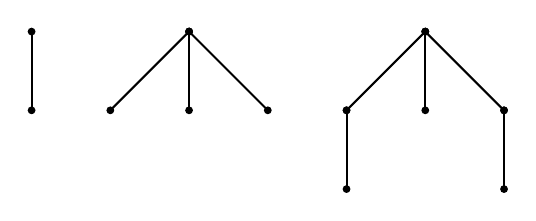
\begin{tikzpicture}
		\draw (0,1)	node[fill,circle, inner sep=1pt] {} -- (0,0) node[fill,circle,inner sep=1pt] {};

		\draw (2,1)	node[fill,circle, inner sep=1pt] {} -- (2,0) node[fill,circle,inner sep=1pt] {};
		\draw (2,1)	node[fill,circle, inner sep=1pt] {} -- (1,0) node[fill,circle,inner sep=1pt] {};
		\draw (2,1)	node[fill,circle, inner sep=1pt] {} -- (3,0) node[fill,circle,inner sep=1pt] {};

		\draw (5,1)	node[fill,circle, inner sep=1pt] {} -- (4,0) node[fill,circle,inner sep=1pt] {};
		\draw (4,0)	node[fill,circle, inner sep=1pt] {} -- (4,-1) node[fill,circle,inner sep=1pt] {};
		\draw (5,1)	node[fill,circle, inner sep=1pt] {} -- (5,0) node[fill,circle,inner sep=1pt] {};
		\draw (5,1)	node[fill,circle, inner sep=1pt] {} -- (6,0) node[fill,circle,inner sep=1pt] {};
		\draw (6,0)	node[fill,circle, inner sep=1pt] {} -- (6,-1) node[fill,circle,inner sep=1pt] {};
	\end{tikzpicture}
	\caption{Foresta ordinata di alberi.}
	\label{fig:ordered_forest}
\end{figure}
Formalmente, definiamo induttivamente una foresta ordinata:
\begin{itemize}
	\item $\langle \rangle$ indica la lista vuota di alberi ed è una foresta ordinata;
	\item se $\langle T_1, \cdots, T_k\rangle$ sono alberi, allora $\langle T_1, \cdots, T_k\rangle$ è una
	      foresta ordinata
	\item se $F$ è una foresta ordinata, $tree(F)$ è un albero radicato in un
	      nuovo nodo che ha come figli tutti gli alberi di $F$.
\end{itemize}

\subsubsection{Isomorfismo tra foreste ordinate e alberi binari}
Definiamo una funzione $\phi$ che associa ad ogni foresta ordinata un preciso albero binario.
Induttivamente,
$$
	\phi(\langle \rangle) = \cdot
$$
ossia $\phi$ di una foresta vuota è un albero costituito da una singola radice.
$$
	\phi(\langle tree(F), T_1, \cdots, T_k>\rangle) = (\phi(F), \phi(\langle T_1, \cdots, T_k\rangle))
$$

\begin{figure}[h]
	\centering
	\tikzset{every picture/.style={line width=0.75pt}} %set default line width to 0.75pt        

	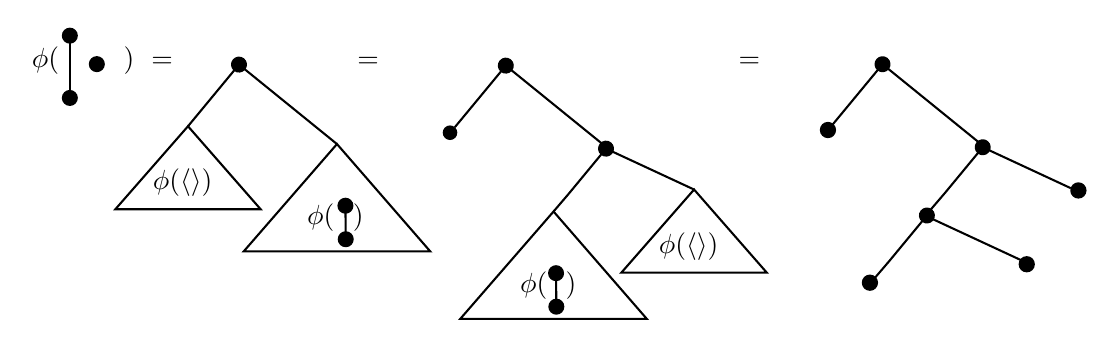
\begin{tikzpicture}[x=0.75pt,y=0.75pt,yscale=-1,xscale=1]
		%uncomment if require: \path (0,300); %set diagram left start at 0, and has height of 300

		%Straight Lines [id:da1467409507063523] 
		\draw    (144.93,41.07) -- (144.93,71.07) ;
		\draw [shift={(144.93,71.07)}, rotate = 90] [color={rgb, 255:red, 0; green, 0; blue, 0 }  ][fill={rgb, 255:red, 0; green, 0; blue, 0 }  ][line width=0.75]      (0, 0) circle [x radius= 3.35, y radius= 3.35]   ;
		\draw [shift={(144.93,41.07)}, rotate = 90] [color={rgb, 255:red, 0; green, 0; blue, 0 }  ][fill={rgb, 255:red, 0; green, 0; blue, 0 }  ][line width=0.75]      (0, 0) circle [x radius= 3.35, y radius= 3.35]   ;
		%Shape: Circle [id:dp48951213847038366] 
		\draw  [fill={rgb, 255:red, 0; green, 0; blue, 0 }  ,fill opacity=1 ] (154.57,54.79) .. controls (154.57,52.93) and (156.07,51.43) .. (157.93,51.43) .. controls (159.78,51.43) and (161.29,52.93) .. (161.29,54.79) .. controls (161.29,56.64) and (159.78,58.14) .. (157.93,58.14) .. controls (156.07,58.14) and (154.57,56.64) .. (154.57,54.79) -- cycle ;

		%Straight Lines [id:da5368285010745462] 
		\draw    (226.43,55) -- (208.31,76.91) -- (201.86,84.71) ;
		\draw [shift={(226.43,55)}, rotate = 129.59] [color={rgb, 255:red, 0; green, 0; blue, 0 }  ][fill={rgb, 255:red, 0; green, 0; blue, 0 }  ][line width=0.75]      (0, 0) circle [x radius= 3.35, y radius= 3.35]   ;
		%Shape: Triangle [id:dp5019688866391238] 
		\draw   (201.86,84.71) -- (236.86,124.71) -- (166.86,124.71) -- cycle ;
		%Shape: Triangle [id:dp12657672899601724] 
		\draw   (273.64,93.29) -- (318.57,145) -- (228.71,145) -- cycle ;
		%Straight Lines [id:da934069022901869] 
		\draw    (226.43,55) -- (273.64,93.29) ;
		%Straight Lines [id:da2898443038516424] 
		\draw    (277.71,123) -- (277.86,139.14) ;
		\draw [shift={(277.86,139.14)}, rotate = 89.49] [color={rgb, 255:red, 0; green, 0; blue, 0 }  ][fill={rgb, 255:red, 0; green, 0; blue, 0 }  ][line width=0.75]      (0, 0) circle [x radius= 3.35, y radius= 3.35]   ;
		\draw [shift={(277.71,123)}, rotate = 89.49] [color={rgb, 255:red, 0; green, 0; blue, 0 }  ][fill={rgb, 255:red, 0; green, 0; blue, 0 }  ][line width=0.75]      (0, 0) circle [x radius= 3.35, y radius= 3.35]   ;
		%Straight Lines [id:da8113066852584067] 
		\draw    (354.98,55.5) -- (336.86,77.41) -- (330.4,85.21) ;
		\draw [shift={(354.98,55.5)}, rotate = 129.59] [color={rgb, 255:red, 0; green, 0; blue, 0 }  ][fill={rgb, 255:red, 0; green, 0; blue, 0 }  ][line width=0.75]      (0, 0) circle [x radius= 3.35, y radius= 3.35]   ;
		%Straight Lines [id:da7241289121021388] 
		\draw    (354.98,55.5) -- (402.19,93.79) ;
		%Shape: Circle [id:dp6494084453696087] 
		\draw  [fill={rgb, 255:red, 0; green, 0; blue, 0 }  ,fill opacity=1 ] (325.1,87.83) .. controls (325.1,86.18) and (326.44,84.83) .. (328.1,84.83) .. controls (329.76,84.83) and (331.1,86.18) .. (331.1,87.83) .. controls (331.1,89.49) and (329.76,90.83) .. (328.1,90.83) .. controls (326.44,90.83) and (325.1,89.49) .. (325.1,87.83) -- cycle ;
		%Straight Lines [id:da4037066529287967] 
		\draw    (403.26,95.5) -- (385.15,117.41) -- (377.98,125.79) ;
		\draw [shift={(403.26,95.5)}, rotate = 129.59] [color={rgb, 255:red, 0; green, 0; blue, 0 }  ][fill={rgb, 255:red, 0; green, 0; blue, 0 }  ][line width=0.75]      (0, 0) circle [x radius= 3.35, y radius= 3.35]   ;
		%Shape: Triangle [id:dp04881880314765141] 
		\draw   (445.69,115.21) -- (480.69,155.21) -- (410.69,155.21) -- cycle ;

		%Shape: Triangle [id:dp12559883893437063] 
		\draw   (377.98,125.79) -- (422.9,177.5) -- (333.05,177.5) -- cycle ;
		%Straight Lines [id:da48087885685526743] 
		\draw    (379.19,155.5) -- (379.33,171.64) ;
		\draw [shift={(379.33,171.64)}, rotate = 89.49] [color={rgb, 255:red, 0; green, 0; blue, 0 }  ][fill={rgb, 255:red, 0; green, 0; blue, 0 }  ][line width=0.75]      (0, 0) circle [x radius= 3.35, y radius= 3.35]   ;
		\draw [shift={(379.19,155.5)}, rotate = 89.49] [color={rgb, 255:red, 0; green, 0; blue, 0 }  ][fill={rgb, 255:red, 0; green, 0; blue, 0 }  ][line width=0.75]      (0, 0) circle [x radius= 3.35, y radius= 3.35]   ;
		%Straight Lines [id:da02388870469608051] 
		\draw    (403.26,95.5) -- (445.69,115.21) ;
		%Straight Lines [id:da6273665141516217] 
		\draw    (536.48,54.83) -- (518.36,76.74) -- (511.9,84.55) ;
		\draw [shift={(536.48,54.83)}, rotate = 129.59] [color={rgb, 255:red, 0; green, 0; blue, 0 }  ][fill={rgb, 255:red, 0; green, 0; blue, 0 }  ][line width=0.75]      (0, 0) circle [x radius= 3.35, y radius= 3.35]   ;
		%Straight Lines [id:da5905284436508569] 
		\draw    (536.48,54.83) -- (583.69,93.12) ;
		%Straight Lines [id:da2030740854922638] 
		\draw    (584.76,94.83) -- (566.65,116.74) -- (559.48,125.12) ;
		\draw [shift={(584.76,94.83)}, rotate = 129.59] [color={rgb, 255:red, 0; green, 0; blue, 0 }  ][fill={rgb, 255:red, 0; green, 0; blue, 0 }  ][line width=0.75]      (0, 0) circle [x radius= 3.35, y radius= 3.35]   ;
		%Straight Lines [id:da49066689108397754] 
		\draw    (584.76,94.83) -- (627.19,114.55) ;
		%Straight Lines [id:da38720603069737713] 
		\draw    (557.87,127.72) -- (539.76,149.63) -- (532.59,158.01) ;
		\draw [shift={(557.87,127.72)}, rotate = 129.59] [color={rgb, 255:red, 0; green, 0; blue, 0 }  ][fill={rgb, 255:red, 0; green, 0; blue, 0 }  ][line width=0.75]      (0, 0) circle [x radius= 3.35, y radius= 3.35]   ;
		%Straight Lines [id:da1048947282900694] 
		\draw    (560.76,129.5) -- (603.19,149.21) ;
		%Shape: Circle [id:dp32417892244375524] 
		\draw  [fill={rgb, 255:red, 0; green, 0; blue, 0 }  ,fill opacity=1 ] (533.82,160.09) .. controls (533.82,158.2) and (532.3,156.67) .. (530.41,156.67) .. controls (528.53,156.67) and (527,158.2) .. (527,160.09) .. controls (527,161.97) and (528.53,163.5) .. (530.41,163.5) .. controls (532.3,163.5) and (533.82,161.97) .. (533.82,160.09) -- cycle ;
		%Shape: Circle [id:dp9675952466326133] 
		\draw  [fill={rgb, 255:red, 0; green, 0; blue, 0 }  ,fill opacity=1 ] (513.6,86.53) .. controls (513.6,84.65) and (512.07,83.12) .. (510.19,83.12) .. controls (508.3,83.12) and (506.78,84.65) .. (506.78,86.53) .. controls (506.78,88.42) and (508.3,89.94) .. (510.19,89.94) .. controls (512.07,89.94) and (513.6,88.42) .. (513.6,86.53) -- cycle ;

		%Shape: Circle [id:dp5658104800173653] 
		\draw  [fill={rgb, 255:red, 0; green, 0; blue, 0 }  ,fill opacity=1 ] (609.38,151.2) .. controls (609.38,149.31) and (607.85,147.79) .. (605.97,147.79) .. controls (604.08,147.79) and (602.55,149.31) .. (602.55,151.2) .. controls (602.55,153.08) and (604.08,154.61) .. (605.97,154.61) .. controls (607.85,154.61) and (609.38,153.08) .. (609.38,151.2) -- cycle ;
		%Shape: Circle [id:dp12193907009892957] 
		\draw  [fill={rgb, 255:red, 0; green, 0; blue, 0 }  ,fill opacity=1 ] (634.27,115.64) .. controls (634.27,113.76) and (632.74,112.23) .. (630.86,112.23) .. controls (628.97,112.23) and (627.44,113.76) .. (627.44,115.64) .. controls (627.44,117.53) and (628.97,119.06) .. (630.86,119.06) .. controls (632.74,119.06) and (634.27,117.53) .. (634.27,115.64) -- cycle ;


		% Text Node
		\draw (125.12,44.91) node [anchor=north west][inner sep=0.75pt]    {$\phi ( \ \ \ \ \ \ \ ) \ =\ \ \ \ \ \ \ \ \ \ \ \ \ \ \ \ \ \ \ \ =\ \ \ \ \ \ \ \ \ \ \ \ \ \ \ \ \ \ \ \ \ \ \ \ \ \ \ \ \ \ \ \ \ \ \ \ \ \ \ =\ $};
		% Text Node
		\draw (427.26,134.33) node [anchor=north west][inner sep=0.75pt]    {$\phi ( \langle \rangle )$};
		% Text Node
		\draw (183.43,103.83) node [anchor=north west][inner sep=0.75pt]    {$\phi ( \langle \rangle )$};
		% Text Node
		\draw (257.75,120.69) node [anchor=north west][inner sep=0.75pt]    {$\phi ( \ \ )$};
		% Text Node
		\draw (360.33,153.19) node [anchor=north west][inner sep=0.75pt]    {$\phi ( \ \ )$};


	\end{tikzpicture}
	\caption{Esempio di calcolo isomorfismo tra foreste e alberi binari.}
	\label{fig:iso_forest_bintree_example}
\end{figure}



\begin{figure}[h]
	\centering



	\tikzset{every picture/.style={line width=0.75pt}} %set default line width to 0.75pt        

	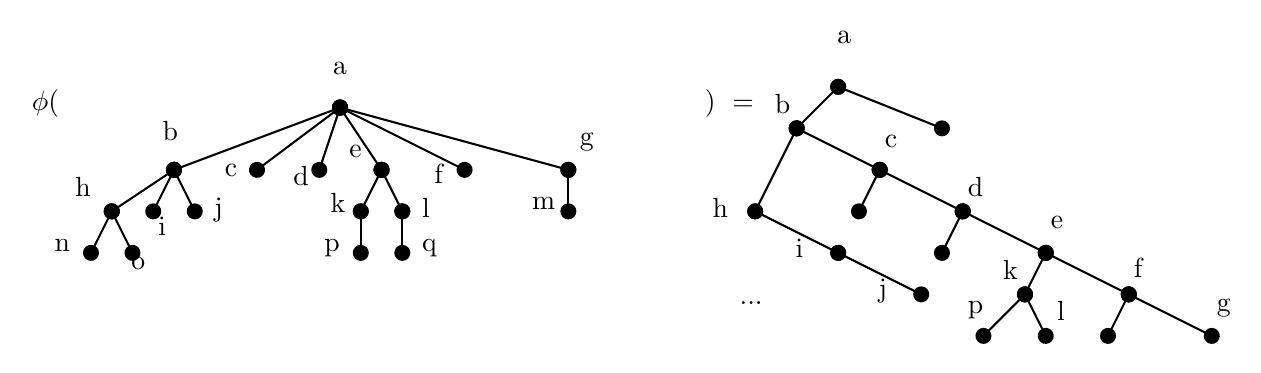
\begin{tikzpicture}[x=0.75pt,y=0.75pt,yscale=-1,xscale=1]
		%uncomment if require: \path (0,300); %set diagram left start at 0, and has height of 300

		%Straight Lines [id:da7390170116429094] 
		\draw    (220,90) -- (330,120) ;
		\draw [shift={(330,120)}, rotate = 15.26] [color={rgb, 255:red, 0; green, 0; blue, 0 }  ][fill={rgb, 255:red, 0; green, 0; blue, 0 }  ][line width=0.75]      (0, 0) circle [x radius= 3.35, y radius= 3.35]   ;
		\draw [shift={(220,90)}, rotate = 15.26] [color={rgb, 255:red, 0; green, 0; blue, 0 }  ][fill={rgb, 255:red, 0; green, 0; blue, 0 }  ][line width=0.75]      (0, 0) circle [x radius= 3.35, y radius= 3.35]   ;
		%Straight Lines [id:da039244879101243746] 
		\draw    (220,90) -- (280,120) ;
		\draw [shift={(280,120)}, rotate = 26.57] [color={rgb, 255:red, 0; green, 0; blue, 0 }  ][fill={rgb, 255:red, 0; green, 0; blue, 0 }  ][line width=0.75]      (0, 0) circle [x radius= 3.35, y radius= 3.35]   ;
		\draw [shift={(220,90)}, rotate = 26.57] [color={rgb, 255:red, 0; green, 0; blue, 0 }  ][fill={rgb, 255:red, 0; green, 0; blue, 0 }  ][line width=0.75]      (0, 0) circle [x radius= 3.35, y radius= 3.35]   ;
		%Straight Lines [id:da9807403722275164] 
		\draw    (220,90) -- (240,120) ;
		\draw [shift={(240,120)}, rotate = 56.31] [color={rgb, 255:red, 0; green, 0; blue, 0 }  ][fill={rgb, 255:red, 0; green, 0; blue, 0 }  ][line width=0.75]      (0, 0) circle [x radius= 3.35, y radius= 3.35]   ;
		\draw [shift={(220,90)}, rotate = 56.31] [color={rgb, 255:red, 0; green, 0; blue, 0 }  ][fill={rgb, 255:red, 0; green, 0; blue, 0 }  ][line width=0.75]      (0, 0) circle [x radius= 3.35, y radius= 3.35]   ;
		%Straight Lines [id:da03267007977703551] 
		\draw    (220,90) -- (210,120) ;
		\draw [shift={(210,120)}, rotate = 108.43] [color={rgb, 255:red, 0; green, 0; blue, 0 }  ][fill={rgb, 255:red, 0; green, 0; blue, 0 }  ][line width=0.75]      (0, 0) circle [x radius= 3.35, y radius= 3.35]   ;
		\draw [shift={(220,90)}, rotate = 108.43] [color={rgb, 255:red, 0; green, 0; blue, 0 }  ][fill={rgb, 255:red, 0; green, 0; blue, 0 }  ][line width=0.75]      (0, 0) circle [x radius= 3.35, y radius= 3.35]   ;
		%Straight Lines [id:da3117293837981189] 
		\draw    (220,90) -- (140,120) ;
		\draw [shift={(140,120)}, rotate = 159.44] [color={rgb, 255:red, 0; green, 0; blue, 0 }  ][fill={rgb, 255:red, 0; green, 0; blue, 0 }  ][line width=0.75]      (0, 0) circle [x radius= 3.35, y radius= 3.35]   ;
		\draw [shift={(220,90)}, rotate = 159.44] [color={rgb, 255:red, 0; green, 0; blue, 0 }  ][fill={rgb, 255:red, 0; green, 0; blue, 0 }  ][line width=0.75]      (0, 0) circle [x radius= 3.35, y radius= 3.35]   ;
		%Straight Lines [id:da5543598400532516] 
		\draw    (220,90) -- (180,120) ;
		\draw [shift={(180,120)}, rotate = 143.13] [color={rgb, 255:red, 0; green, 0; blue, 0 }  ][fill={rgb, 255:red, 0; green, 0; blue, 0 }  ][line width=0.75]      (0, 0) circle [x radius= 3.35, y radius= 3.35]   ;
		\draw [shift={(220,90)}, rotate = 143.13] [color={rgb, 255:red, 0; green, 0; blue, 0 }  ][fill={rgb, 255:red, 0; green, 0; blue, 0 }  ][line width=0.75]      (0, 0) circle [x radius= 3.35, y radius= 3.35]   ;
		%Straight Lines [id:da6616928412892461] 
		\draw    (140,120) -- (130,140) ;
		\draw [shift={(130,140)}, rotate = 116.57] [color={rgb, 255:red, 0; green, 0; blue, 0 }  ][fill={rgb, 255:red, 0; green, 0; blue, 0 }  ][line width=0.75]      (0, 0) circle [x radius= 3.35, y radius= 3.35]   ;
		\draw [shift={(140,120)}, rotate = 116.57] [color={rgb, 255:red, 0; green, 0; blue, 0 }  ][fill={rgb, 255:red, 0; green, 0; blue, 0 }  ][line width=0.75]      (0, 0) circle [x radius= 3.35, y radius= 3.35]   ;
		%Straight Lines [id:da5001878304038733] 
		\draw    (140,120) -- (110,140) ;
		\draw [shift={(110,140)}, rotate = 146.31] [color={rgb, 255:red, 0; green, 0; blue, 0 }  ][fill={rgb, 255:red, 0; green, 0; blue, 0 }  ][line width=0.75]      (0, 0) circle [x radius= 3.35, y radius= 3.35]   ;
		\draw [shift={(140,120)}, rotate = 146.31] [color={rgb, 255:red, 0; green, 0; blue, 0 }  ][fill={rgb, 255:red, 0; green, 0; blue, 0 }  ][line width=0.75]      (0, 0) circle [x radius= 3.35, y radius= 3.35]   ;
		%Straight Lines [id:da35297443192918876] 
		\draw    (140,120) -- (150,140) ;
		\draw [shift={(150,140)}, rotate = 63.43] [color={rgb, 255:red, 0; green, 0; blue, 0 }  ][fill={rgb, 255:red, 0; green, 0; blue, 0 }  ][line width=0.75]      (0, 0) circle [x radius= 3.35, y radius= 3.35]   ;
		\draw [shift={(140,120)}, rotate = 63.43] [color={rgb, 255:red, 0; green, 0; blue, 0 }  ][fill={rgb, 255:red, 0; green, 0; blue, 0 }  ][line width=0.75]      (0, 0) circle [x radius= 3.35, y radius= 3.35]   ;
		%Straight Lines [id:da30077845664351066] 
		\draw    (110,140) -- (100,160) ;
		\draw [shift={(100,160)}, rotate = 116.57] [color={rgb, 255:red, 0; green, 0; blue, 0 }  ][fill={rgb, 255:red, 0; green, 0; blue, 0 }  ][line width=0.75]      (0, 0) circle [x radius= 3.35, y radius= 3.35]   ;
		\draw [shift={(110,140)}, rotate = 116.57] [color={rgb, 255:red, 0; green, 0; blue, 0 }  ][fill={rgb, 255:red, 0; green, 0; blue, 0 }  ][line width=0.75]      (0, 0) circle [x radius= 3.35, y radius= 3.35]   ;
		%Straight Lines [id:da5436015840206943] 
		\draw    (110,140) -- (120,160) ;
		\draw [shift={(120,160)}, rotate = 63.43] [color={rgb, 255:red, 0; green, 0; blue, 0 }  ][fill={rgb, 255:red, 0; green, 0; blue, 0 }  ][line width=0.75]      (0, 0) circle [x radius= 3.35, y radius= 3.35]   ;
		\draw [shift={(110,140)}, rotate = 63.43] [color={rgb, 255:red, 0; green, 0; blue, 0 }  ][fill={rgb, 255:red, 0; green, 0; blue, 0 }  ][line width=0.75]      (0, 0) circle [x radius= 3.35, y radius= 3.35]   ;
		%Straight Lines [id:da3418649793206039] 
		\draw    (240,120) -- (230,140) ;
		\draw [shift={(230,140)}, rotate = 116.57] [color={rgb, 255:red, 0; green, 0; blue, 0 }  ][fill={rgb, 255:red, 0; green, 0; blue, 0 }  ][line width=0.75]      (0, 0) circle [x radius= 3.35, y radius= 3.35]   ;
		\draw [shift={(240,120)}, rotate = 116.57] [color={rgb, 255:red, 0; green, 0; blue, 0 }  ][fill={rgb, 255:red, 0; green, 0; blue, 0 }  ][line width=0.75]      (0, 0) circle [x radius= 3.35, y radius= 3.35]   ;
		%Straight Lines [id:da5537357380053466] 
		\draw    (240,120) -- (250,140) ;
		\draw [shift={(250,140)}, rotate = 63.43] [color={rgb, 255:red, 0; green, 0; blue, 0 }  ][fill={rgb, 255:red, 0; green, 0; blue, 0 }  ][line width=0.75]      (0, 0) circle [x radius= 3.35, y radius= 3.35]   ;
		\draw [shift={(240,120)}, rotate = 63.43] [color={rgb, 255:red, 0; green, 0; blue, 0 }  ][fill={rgb, 255:red, 0; green, 0; blue, 0 }  ][line width=0.75]      (0, 0) circle [x radius= 3.35, y radius= 3.35]   ;
		%Straight Lines [id:da596511628614987] 
		\draw    (330,120) -- (330,140) ;
		\draw [shift={(330,140)}, rotate = 90] [color={rgb, 255:red, 0; green, 0; blue, 0 }  ][fill={rgb, 255:red, 0; green, 0; blue, 0 }  ][line width=0.75]      (0, 0) circle [x radius= 3.35, y radius= 3.35]   ;
		\draw [shift={(330,120)}, rotate = 90] [color={rgb, 255:red, 0; green, 0; blue, 0 }  ][fill={rgb, 255:red, 0; green, 0; blue, 0 }  ][line width=0.75]      (0, 0) circle [x radius= 3.35, y radius= 3.35]   ;
		%Straight Lines [id:da9692313360351018] 
		\draw    (250,140) -- (250,160) ;
		\draw [shift={(250,160)}, rotate = 90] [color={rgb, 255:red, 0; green, 0; blue, 0 }  ][fill={rgb, 255:red, 0; green, 0; blue, 0 }  ][line width=0.75]      (0, 0) circle [x radius= 3.35, y radius= 3.35]   ;
		\draw [shift={(250,140)}, rotate = 90] [color={rgb, 255:red, 0; green, 0; blue, 0 }  ][fill={rgb, 255:red, 0; green, 0; blue, 0 }  ][line width=0.75]      (0, 0) circle [x radius= 3.35, y radius= 3.35]   ;
		%Straight Lines [id:da3464424144057545] 
		\draw    (230,140) -- (230,160) ;
		\draw [shift={(230,160)}, rotate = 90] [color={rgb, 255:red, 0; green, 0; blue, 0 }  ][fill={rgb, 255:red, 0; green, 0; blue, 0 }  ][line width=0.75]      (0, 0) circle [x radius= 3.35, y radius= 3.35]   ;
		\draw [shift={(230,140)}, rotate = 90] [color={rgb, 255:red, 0; green, 0; blue, 0 }  ][fill={rgb, 255:red, 0; green, 0; blue, 0 }  ][line width=0.75]      (0, 0) circle [x radius= 3.35, y radius= 3.35]   ;
		%Straight Lines [id:da9449001958581409] 
		\draw    (460,80) -- (510,100) ;
		\draw [shift={(510,100)}, rotate = 21.8] [color={rgb, 255:red, 0; green, 0; blue, 0 }  ][fill={rgb, 255:red, 0; green, 0; blue, 0 }  ][line width=0.75]      (0, 0) circle [x radius= 3.35, y radius= 3.35]   ;
		\draw [shift={(460,80)}, rotate = 21.8] [color={rgb, 255:red, 0; green, 0; blue, 0 }  ][fill={rgb, 255:red, 0; green, 0; blue, 0 }  ][line width=0.75]      (0, 0) circle [x radius= 3.35, y radius= 3.35]   ;
		%Straight Lines [id:da5101057369964663] 
		\draw    (460,80) -- (440,100) ;
		\draw [shift={(440,100)}, rotate = 135] [color={rgb, 255:red, 0; green, 0; blue, 0 }  ][fill={rgb, 255:red, 0; green, 0; blue, 0 }  ][line width=0.75]      (0, 0) circle [x radius= 3.35, y radius= 3.35]   ;
		\draw [shift={(460,80)}, rotate = 135] [color={rgb, 255:red, 0; green, 0; blue, 0 }  ][fill={rgb, 255:red, 0; green, 0; blue, 0 }  ][line width=0.75]      (0, 0) circle [x radius= 3.35, y radius= 3.35]   ;
		%Straight Lines [id:da7168760346038819] 
		\draw    (440,100) -- (480,120) ;
		\draw [shift={(480,120)}, rotate = 26.57] [color={rgb, 255:red, 0; green, 0; blue, 0 }  ][fill={rgb, 255:red, 0; green, 0; blue, 0 }  ][line width=0.75]      (0, 0) circle [x radius= 3.35, y radius= 3.35]   ;
		\draw [shift={(440,100)}, rotate = 26.57] [color={rgb, 255:red, 0; green, 0; blue, 0 }  ][fill={rgb, 255:red, 0; green, 0; blue, 0 }  ][line width=0.75]      (0, 0) circle [x radius= 3.35, y radius= 3.35]   ;
		%Straight Lines [id:da7536172846092781] 
		\draw    (480,120) -- (520,140) ;
		\draw [shift={(520,140)}, rotate = 26.57] [color={rgb, 255:red, 0; green, 0; blue, 0 }  ][fill={rgb, 255:red, 0; green, 0; blue, 0 }  ][line width=0.75]      (0, 0) circle [x radius= 3.35, y radius= 3.35]   ;
		\draw [shift={(480,120)}, rotate = 26.57] [color={rgb, 255:red, 0; green, 0; blue, 0 }  ][fill={rgb, 255:red, 0; green, 0; blue, 0 }  ][line width=0.75]      (0, 0) circle [x radius= 3.35, y radius= 3.35]   ;
		%Straight Lines [id:da06546573584424464] 
		\draw    (520,140) -- (560,160) ;
		\draw [shift={(560,160)}, rotate = 26.57] [color={rgb, 255:red, 0; green, 0; blue, 0 }  ][fill={rgb, 255:red, 0; green, 0; blue, 0 }  ][line width=0.75]      (0, 0) circle [x radius= 3.35, y radius= 3.35]   ;
		\draw [shift={(520,140)}, rotate = 26.57] [color={rgb, 255:red, 0; green, 0; blue, 0 }  ][fill={rgb, 255:red, 0; green, 0; blue, 0 }  ][line width=0.75]      (0, 0) circle [x radius= 3.35, y radius= 3.35]   ;
		%Straight Lines [id:da31121333233660786] 
		\draw    (560,160) -- (600,180) ;
		\draw [shift={(600,180)}, rotate = 26.57] [color={rgb, 255:red, 0; green, 0; blue, 0 }  ][fill={rgb, 255:red, 0; green, 0; blue, 0 }  ][line width=0.75]      (0, 0) circle [x radius= 3.35, y radius= 3.35]   ;
		\draw [shift={(560,160)}, rotate = 26.57] [color={rgb, 255:red, 0; green, 0; blue, 0 }  ][fill={rgb, 255:red, 0; green, 0; blue, 0 }  ][line width=0.75]      (0, 0) circle [x radius= 3.35, y radius= 3.35]   ;
		%Straight Lines [id:da9734645903114482] 
		\draw    (600,180) -- (640,200) ;
		\draw [shift={(640,200)}, rotate = 26.57] [color={rgb, 255:red, 0; green, 0; blue, 0 }  ][fill={rgb, 255:red, 0; green, 0; blue, 0 }  ][line width=0.75]      (0, 0) circle [x radius= 3.35, y radius= 3.35]   ;
		\draw [shift={(600,180)}, rotate = 26.57] [color={rgb, 255:red, 0; green, 0; blue, 0 }  ][fill={rgb, 255:red, 0; green, 0; blue, 0 }  ][line width=0.75]      (0, 0) circle [x radius= 3.35, y radius= 3.35]   ;
		%Straight Lines [id:da3400373607542443] 
		\draw    (480,120) -- (470,140) ;
		\draw [shift={(470,140)}, rotate = 116.57] [color={rgb, 255:red, 0; green, 0; blue, 0 }  ][fill={rgb, 255:red, 0; green, 0; blue, 0 }  ][line width=0.75]      (0, 0) circle [x radius= 3.35, y radius= 3.35]   ;
		\draw [shift={(480,120)}, rotate = 116.57] [color={rgb, 255:red, 0; green, 0; blue, 0 }  ][fill={rgb, 255:red, 0; green, 0; blue, 0 }  ][line width=0.75]      (0, 0) circle [x radius= 3.35, y radius= 3.35]   ;
		%Straight Lines [id:da8071946852447195] 
		\draw    (520,140) -- (510,160) ;
		\draw [shift={(510,160)}, rotate = 116.57] [color={rgb, 255:red, 0; green, 0; blue, 0 }  ][fill={rgb, 255:red, 0; green, 0; blue, 0 }  ][line width=0.75]      (0, 0) circle [x radius= 3.35, y radius= 3.35]   ;
		\draw [shift={(520,140)}, rotate = 116.57] [color={rgb, 255:red, 0; green, 0; blue, 0 }  ][fill={rgb, 255:red, 0; green, 0; blue, 0 }  ][line width=0.75]      (0, 0) circle [x radius= 3.35, y radius= 3.35]   ;
		%Straight Lines [id:da9920119862914486] 
		\draw    (600,180) -- (590,200) ;
		\draw [shift={(590,200)}, rotate = 116.57] [color={rgb, 255:red, 0; green, 0; blue, 0 }  ][fill={rgb, 255:red, 0; green, 0; blue, 0 }  ][line width=0.75]      (0, 0) circle [x radius= 3.35, y radius= 3.35]   ;
		\draw [shift={(600,180)}, rotate = 116.57] [color={rgb, 255:red, 0; green, 0; blue, 0 }  ][fill={rgb, 255:red, 0; green, 0; blue, 0 }  ][line width=0.75]      (0, 0) circle [x radius= 3.35, y radius= 3.35]   ;
		%Straight Lines [id:da6764843933308277] 
		\draw    (560,160) -- (550,180) ;
		\draw [shift={(550,180)}, rotate = 116.57] [color={rgb, 255:red, 0; green, 0; blue, 0 }  ][fill={rgb, 255:red, 0; green, 0; blue, 0 }  ][line width=0.75]      (0, 0) circle [x radius= 3.35, y radius= 3.35]   ;
		\draw [shift={(560,160)}, rotate = 116.57] [color={rgb, 255:red, 0; green, 0; blue, 0 }  ][fill={rgb, 255:red, 0; green, 0; blue, 0 }  ][line width=0.75]      (0, 0) circle [x radius= 3.35, y radius= 3.35]   ;
		%Straight Lines [id:da9822121216527463] 
		\draw    (550,180) -- (530,200) ;
		\draw [shift={(530,200)}, rotate = 135] [color={rgb, 255:red, 0; green, 0; blue, 0 }  ][fill={rgb, 255:red, 0; green, 0; blue, 0 }  ][line width=0.75]      (0, 0) circle [x radius= 3.35, y radius= 3.35]   ;
		\draw [shift={(550,180)}, rotate = 135] [color={rgb, 255:red, 0; green, 0; blue, 0 }  ][fill={rgb, 255:red, 0; green, 0; blue, 0 }  ][line width=0.75]      (0, 0) circle [x radius= 3.35, y radius= 3.35]   ;
		%Straight Lines [id:da3765788262191845] 
		\draw    (550,180) -- (560,200) ;
		\draw [shift={(560,200)}, rotate = 63.43] [color={rgb, 255:red, 0; green, 0; blue, 0 }  ][fill={rgb, 255:red, 0; green, 0; blue, 0 }  ][line width=0.75]      (0, 0) circle [x radius= 3.35, y radius= 3.35]   ;
		\draw [shift={(550,180)}, rotate = 63.43] [color={rgb, 255:red, 0; green, 0; blue, 0 }  ][fill={rgb, 255:red, 0; green, 0; blue, 0 }  ][line width=0.75]      (0, 0) circle [x radius= 3.35, y radius= 3.35]   ;
		%Straight Lines [id:da057732075656578896] 
		\draw    (420,140) -- (460,160) ;
		\draw [shift={(460,160)}, rotate = 26.57] [color={rgb, 255:red, 0; green, 0; blue, 0 }  ][fill={rgb, 255:red, 0; green, 0; blue, 0 }  ][line width=0.75]      (0, 0) circle [x radius= 3.35, y radius= 3.35]   ;
		\draw [shift={(420,140)}, rotate = 26.57] [color={rgb, 255:red, 0; green, 0; blue, 0 }  ][fill={rgb, 255:red, 0; green, 0; blue, 0 }  ][line width=0.75]      (0, 0) circle [x radius= 3.35, y radius= 3.35]   ;
		%Straight Lines [id:da6702517354459413] 
		\draw    (460,160) -- (500,180) ;
		\draw [shift={(500,180)}, rotate = 26.57] [color={rgb, 255:red, 0; green, 0; blue, 0 }  ][fill={rgb, 255:red, 0; green, 0; blue, 0 }  ][line width=0.75]      (0, 0) circle [x radius= 3.35, y radius= 3.35]   ;
		\draw [shift={(460,160)}, rotate = 26.57] [color={rgb, 255:red, 0; green, 0; blue, 0 }  ][fill={rgb, 255:red, 0; green, 0; blue, 0 }  ][line width=0.75]      (0, 0) circle [x radius= 3.35, y radius= 3.35]   ;
		%Straight Lines [id:da6027456046960759] 
		\draw    (440,100) -- (420,140) ;
		\draw [shift={(420,140)}, rotate = 116.57] [color={rgb, 255:red, 0; green, 0; blue, 0 }  ][fill={rgb, 255:red, 0; green, 0; blue, 0 }  ][line width=0.75]      (0, 0) circle [x radius= 3.35, y radius= 3.35]   ;
		\draw [shift={(440,100)}, rotate = 116.57] [color={rgb, 255:red, 0; green, 0; blue, 0 }  ][fill={rgb, 255:red, 0; green, 0; blue, 0 }  ][line width=0.75]      (0, 0) circle [x radius= 3.35, y radius= 3.35]   ;

		% Text Node
		\draw (70,80) node [anchor=north west][inner sep=0.75pt]    {$\phi ( \ \ \ \ \ \ \ \ \ \ \ \ \ \ \ \ \ \ \ \ \ \ \ \ \ \ \ \ \ \ \ \ \ \ \ \ \ \ \ \ \ \ \ \ \ \ \ \ \ \ \ \ \ \ \ \ \ \ \ \ \ \ \ \ \ \ \ \ \ \ ) \ =\ $};
		% Text Node
		\draw (215,67) node [anchor=north west][inner sep=0.75pt]   [align=left] {a};
		% Text Node
		\draw (133,95) node [anchor=north west][inner sep=0.75pt]   [align=left] {b};
		% Text Node
		\draw (163,116) node [anchor=north west][inner sep=0.75pt]   [align=left] {c};
		% Text Node
		\draw (196,117) node [anchor=north west][inner sep=0.75pt]   [align=left] {d};
		% Text Node
		\draw (223,107) node [anchor=north west][inner sep=0.75pt]   [align=left] {e};
		% Text Node
		\draw (264,116) node [anchor=north west][inner sep=0.75pt]   [align=left] {f};
		% Text Node
		\draw (334,101) node [anchor=north west][inner sep=0.75pt]   [align=left] {g};
		% Text Node
		\draw (91,122) node [anchor=north west][inner sep=0.75pt]   [align=left] {h};
		% Text Node
		\draw (131,141) node [anchor=north west][inner sep=0.75pt]   [align=left] {i};
		% Text Node
		\draw (158,132) node [anchor=north west][inner sep=0.75pt]   [align=left] {j};
		% Text Node
		\draw (214,130) node [anchor=north west][inner sep=0.75pt]   [align=left] {k};
		% Text Node
		\draw (258,132) node [anchor=north west][inner sep=0.75pt]   [align=left] {l};
		% Text Node
		\draw (311,132) node [anchor=north west][inner sep=0.75pt]   [align=left] {m};
		% Text Node
		\draw (81,152) node [anchor=north west][inner sep=0.75pt]   [align=left] {n};
		% Text Node
		\draw (118,161) node [anchor=north west][inner sep=0.75pt]   [align=left] {o};
		% Text Node
		\draw (211,152) node [anchor=north west][inner sep=0.75pt]   [align=left] {p};
		% Text Node
		\draw (258,152) node [anchor=north west][inner sep=0.75pt]   [align=left] {q};
		% Text Node
		\draw (458,52) node [anchor=north west][inner sep=0.75pt]   [align=left] {a};
		% Text Node
		\draw (428,82) node [anchor=north west][inner sep=0.75pt]   [align=left] {b};
		% Text Node
		\draw (481,102) node [anchor=north west][inner sep=0.75pt]   [align=left] {c};
		% Text Node
		\draw (521,122) node [anchor=north west][inner sep=0.75pt]   [align=left] {d};
		% Text Node
		\draw (561,141) node [anchor=north west][inner sep=0.75pt]   [align=left] {e};
		% Text Node
		\draw (601,161) node [anchor=north west][inner sep=0.75pt]   [align=left] {f};
		% Text Node
		\draw (641,181) node [anchor=north west][inner sep=0.75pt]   [align=left] {g};
		% Text Node
		\draw (538,162) node [anchor=north west][inner sep=0.75pt]   [align=left] {k};
		% Text Node
		\draw (521,182) node [anchor=north west][inner sep=0.75pt]   [align=left] {p};
		% Text Node
		\draw (564,182) node [anchor=north west][inner sep=0.75pt]   [align=left] {l};
		% Text Node
		\draw (398,132) node [anchor=north west][inner sep=0.75pt]   [align=left] {h};
		% Text Node
		\draw (438,152) node [anchor=north west][inner sep=0.75pt]   [align=left] {i};
		% Text Node
		\draw (478,171) node [anchor=north west][inner sep=0.75pt]   [align=left] {j};
		% Text Node
		\draw (411,182) node [anchor=north west][inner sep=0.75pt]   [align=left] {...};
	\end{tikzpicture}
	\caption{Funzionamento, in generale, dell'isomorfismo tra foreste ordinate e alberi binari con
		la tecnica `first-child next-sibling`.}
	\label{fig:iso_forest_bintree}
\end{figure}

Ciò che abbiamo dimostrato è che le foreste ordinate sono tante quante gli alberi binari:
$\phi$ `manda' una foresta ordinata con $n$ nodi interni in un albero binario con altrettanti nodi.

\subsubsection{Isomorfismo tra foreste ordinate e parole di Dyck.}
Definiamo $\psi: D_{2n} \rightarrow F_n$ un isomorfismo tra parole ben parentesizzate di lunghezza $2n$ e
foreste ordinate con $n$ nodi induttivamente:
$$
	\psi(\epsilon) = \langle \rangle
$$
$$
	\psi(w_1 \cdots w_k) =  \langle\psi(w_1), \cdots, \psi(w_k)\rangle
$$
e
$$
	\psi((w)) = \langle \text{ albero radicato con figli tutti e soli gli alberi della foresta} \phi(w)  \rangle
$$

\noindent
Sappiamo che $D_{2n} \approxeq F_n \approxeq B_n$ e sappiamo quanti sono i possibili alberi binari
con $n$ nodi grazie al numero di Catalano, sono $|B_n| = C_n  \approx 2n + o (\log_2(n))$; di conseguenza,
le parole di Dyck di lunghezza $2n$ hanno come information-theoretical lower bound
$$
	Z_n = n + o(\log_2(n)) \text{ bit}
$$
Quindi
$$
	D_n - Z_n =  8n + o(n) - n - o(\log_2(n)) = 7n - o(n) - o(\log_2(n))  = O(n) \implies D_n \approx Z_n + O(Z_n)
$$
pertanto la struttura descritta è compatta.

\section{Struttura per hash minimali perfetti}
\subsection{Funzioni di hash}
Le funzioni di hash compaiono in molti contesti diversi e un'applicazione
`famosa' sono le \textit{tabelle di hash}.
Nel modo più generale, dato un universo $U$ infinito o \textit{molto grande} e un numero $m \in \mathbb{N}$,
che è il \textit{numero di bucket}, una funzione di hash è
$$
	h: U \rightarrow m
$$

Le funzioni di hash, che denominiamo $H_{U,m}$, sono infinite se $U$ è infinito, mentre sono finite
se $U$ è finito, in particolare $|H_{U,m}| = m^{|U|}$.
La funzione $h$ deve avere alcune proprietà: prendiamo come esempio proprio le tabelle di hash,
utilizzate per memorizzare un sottoinsieme $S \subseteq U$, per esempio delle stringhe su un certo
alfabeto $\Sigma = \{a, b, c, d\}$. Fissato un $m \in \mathbb{N}$, la funzione è
$$
	h: \Sigma^* \leadsto m
$$
vedendo i simboli in $\Sigma$ come un'enumerazione $a = 0, b = 1, c =2, d = 3$,
una funzione di hash potrebbe semplicemente sommare i simboli di una stringa e
operarne il modulo in $m$, in modo che il valore risultante sia $0 \leq h \le m-1 $.

Lo scopo è mantenere una tabella, spesso realizzata come un vettore di liste di
elementi, i cui indici sono esattamente gli hash possibili che la funzione $h$
calcola. In questo modo, è possibile accedere (quasi) direttamente alle
parole nella tabella\footnote{Vi sono principalmente due modi per costruire
	tabelle di hash: \textit{open addressing} e \textit{separate chaining}.
	In questo frangente stiamo analizzando la versione con separate chaining.}.
In termini pratici, partendo da una tabella vuota, quando
si vuole inserire una stringa $s = "foo"$ nella tabella, si utilizza la funzione
di hash per calcolare $h(s) = h_1$. Il valore calcolato sarà l'indice della
tabella dove inserire il riferimento alla stringa.

\begin{figure}[h]
	\centering
	\tikzset{every picture/.style={line width=0.75pt}} %set default line width to 0.75pt        

	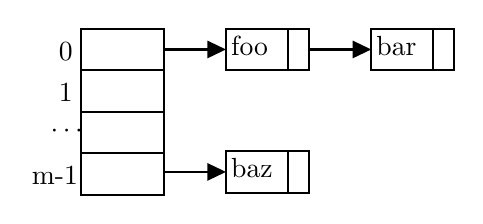
\begin{tikzpicture}[x=0.75pt,y=0.75pt,yscale=-1,xscale=1]
		%uncomment if require: \path (0,300); %set diagram left start at 0, and has height of 300

		%Shape: Rectangle [id:dp9579578997678553] 
		\draw   (70,100) -- (110,100) -- (110,120) -- (70,120) -- cycle ;
		%Shape: Rectangle [id:dp027628855530104857] 
		\draw   (70,80) -- (110,80) -- (110,100) -- (70,100) -- cycle ;
		%Shape: Rectangle [id:dp8143559001814539] 
		\draw   (70,140) -- (110,140) -- (110,160) -- (70,160) -- cycle ;
		%Shape: Rectangle [id:dp38276393364199424] 
		\draw   (70,120) -- (110,120) -- (110,140) -- (70,140) -- cycle ;
		%Straight Lines [id:da801581038753237] 
		\draw    (110,90) -- (137,90) ;
		\draw [shift={(140,90)}, rotate = 180] [fill={rgb, 255:red, 0; green, 0; blue, 0 }  ][line width=0.08]  [draw opacity=0] (8.93,-4.29) -- (0,0) -- (8.93,4.29) -- cycle    ;
		%Shape: Rectangle [id:dp3050844046907898] 
		\draw   (140,80) -- (180,80) -- (180,100) -- (140,100) -- cycle ;
		%Shape: Rectangle [id:dp41513696416167833] 
		\draw   (170,80) -- (180,80) -- (180,100) -- (170,100) -- cycle ;

		%Shape: Rectangle [id:dp43239961582118536] 
		\draw   (210,80) -- (250,80) -- (250,100) -- (210,100) -- cycle ;
		%Shape: Rectangle [id:dp38503115889664563] 
		\draw   (240,80) -- (250,80) -- (250,100) -- (240,100) -- cycle ;

		%Straight Lines [id:da3303160944704562] 
		\draw    (180,90) -- (207,90) ;
		\draw [shift={(210,90)}, rotate = 180] [fill={rgb, 255:red, 0; green, 0; blue, 0 }  ][line width=0.08]  [draw opacity=0] (8.93,-4.29) -- (0,0) -- (8.93,4.29) -- cycle    ;
		%Straight Lines [id:da047149376903893425] 
		\draw    (110,149) -- (137,149) ;
		\draw [shift={(140,149)}, rotate = 180] [fill={rgb, 255:red, 0; green, 0; blue, 0 }  ][line width=0.08]  [draw opacity=0] (8.93,-4.29) -- (0,0) -- (8.93,4.29) -- cycle    ;
		%Shape: Rectangle [id:dp591261104910037] 
		\draw   (140,139) -- (180,139) -- (180,159) -- (140,159) -- cycle ;
		%Shape: Rectangle [id:dp4443187367264515] 
		\draw   (170,139) -- (180,139) -- (180,159) -- (170,159) -- cycle ;


		% Text Node
		\draw (58,85) node [anchor=north west][inner sep=0.75pt]   [align=left] {0};
		% Text Node
		\draw (58,105) node [anchor=north west][inner sep=0.75pt]   [align=left] {1};
		% Text Node
		\draw (54,125) node [anchor=north west][inner sep=0.75pt]   [align=left] {$\displaystyle \cdots $};
		% Text Node
		\draw (45,145) node [anchor=north west][inner sep=0.75pt]   [align=left] {m-1};
		% Text Node
		\draw (141,82) node [anchor=north west][inner sep=0.75pt]   [align=left] {foo};
		% Text Node
		\draw (211,82) node [anchor=north west][inner sep=0.75pt]   [align=left] {bar};
		% Text Node
		\draw (141,141) node [anchor=north west][inner sep=0.75pt]   [align=left] {baz};
	\end{tikzpicture}
	\caption{Esempio di una tabella di hash con separate chaining.}
	\label{fig:hashtable_example}
\end{figure}

Possono accadere dei conflitti, ossia due stringhe $s_1$ e $s_2$ tali che
$h(s_1) = h(s_2)$; per ovviare a questo problema si descrive $M$ come una mappa di liste, ossia
ad un indice $h_1$ di $M$ corrisponde una lista di stringhe.

\subsubsection{Requisiti}
La tabella $M$ funziona con qualsiasi funzione di hash $h$ (anche $h(\cdot) = 0$),
ma l'efficienza di $M$ cambia al suo variare, fino al denegenerare in una lista.
Per far funzionare ``bene'' $M$ è necessario che
\begin{itemize}
	\setlength\itemsep{0pt}
	\item $h$ sia veloce da calcolare; e
	\item $h$ divida l'universo $U$ in \textit{buckets} in modo tale che le
	      controimmagini siano più o meno \textit{grandi uguali}.
	      In altri termini, se guardiamo $\Sigma^*$ e guardiamo come
	      $h$ ne partiziona gli elementi, vorremmo che i blocchi (o bucket)
	      della partizione siano più o meno grandi uguali e non ci sia
	      qualche blocco che contiene molti più elementi degli
	      altri.
	      % disegno pagina 1 15-12-2021 buckets nell'universo. 
\end{itemize}
Questi requisiti sono esprimibili formalmente ovviamente, ma solitamente oltre
a questi requisiti di base ve ne sono altri che dipendono dall'utilizzo
che si vuole fare della funzione; nel nostro caso, facciamo le seguenti
assunzioni: la prima, chiamata \textit{full randomness assumption},
è che possiamo estrarre uniformemente una funzione $h$ dall'insieme $\mathcal{H}_{U,m}$.

La seconda è che $h$ sia calcolabile in tempo e spazio costante, inoltre occupa
spazio costante in termini di codice (non usa array arbitrariamente grandi, ...).
Questa assunzione è normalmente inattuabile: si pensi al caso in cui $U = \Sigma^*$:
si dovrebbero considerare tutte le possibili funzioni dalle stringhe ai naturali
minori di $m$, che sono infinite e tra le quali ce ne sono anche di non calcolabili.

\subsubsection{Rappresentazione}
Ciò che si può fare è invece considerare un universo limitato con un
upper bound dipendente da un qualche intero $k$.
Chiaramente si perde della `randomness', ma il vantaggio è che molto spesso
i risultati che si ottengono sotto l'assunzione di completa casualità si possono
portare anche sotto $U$ così definito, magari con qualche approssimazione.

Supponiamo quindi di avere $U = \Sigma^{\leq k}$; vogliamo scrivere delle
funzioni $h: U \rightarrow m$, alcune di esse possono essere descritte nel
seguente modo.
Si usa un array $\mathbf{p}$ chiamato \textit{array dei pesi} contenente $k$ valori,
inizializzandolo a valori pseudocasuali nell'insieme $\{0, \cdots, m-1\}$.
Quando si vuole calcolare l'hash di una stringa $s = "foo"$ si considera il valore
di ogni lettera della stringa e si moltiplica per il peso di quel carattere
in senso posizionale, ossia il primo peso è associato al primo carattere della stringa,
il secondo peso al secondo carattere e così via; quindi si sommano i risultati e
si computa il modulo $m$. Per esempio, se
$$
	a = 0, b = 1, c = 2, \cdots, f = 5, \cdots, o = 14, \cdots
$$
e
$$
	\mathbf{p} = [15, 86, 90, \cdots]
$$
Il calcolo dell'hash è
$$
	h("foo") = ((5 * 15) + (14 * 86) + (14*90)) \mod m
$$
ottendo un valore che si calcola in un tempo lineare nella lunghezza della stringa
diverso per ogni possibile scelta dei pesi. Cioè, non stiamo
scegliendo tra tutte le possibili funzioni di hash, bensì scegliamo tra le funzioni
di hash caratterizzabili dal vettore $\mathbf{p}$, ossia in $m^k$ modi.
Queste funzioni non occupano molto spazio e si calcolano in un tempo non
costante ma logaritmico nella dimensione dell'universo.

\subsection{Relazione con i grafi}
\subsubsection{Sequenza di peeling di un grafo}
Si supponga di avere un grafo $G = (V,E)$ non orientato. Una \textbf{sequenza di peeling} è
una sequenza di coppie di archi e vertici in cui appaiono tutti i lati e uno dei
due vertici incidenti a tale lato. Ogni vertice che appare è chiamato \textit{hinge}
della sequenza. La sequenza deve essere tale per cui nessun vertice hinge $x_i$
è apparso nei lati che precedono $i$.

\begin{figure}[htpb]
	\begin{center}
		\begin{subfigure}[b]{0.45\textwidth}
			\begin{center}
				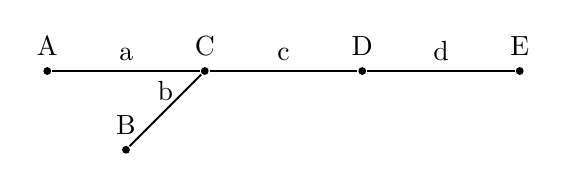
\begin{tikzpicture}
					\node [circle,fill,label=above:{A},inner sep=1pt](A) at (0,0) {};
					\node [circle,fill,label=above:{B},inner sep=1pt](B) at (1,-1) {};
					\node [circle,fill,label=above:{C},inner sep=1pt](C) at (2,0) {};
					\node [circle,fill,label=above:{D},inner sep=1pt](D) at (4,0) {};
					\node [circle,fill,label=above:{E},inner sep=1pt](E) at (6,0) {};

					\draw (A) -- (C) node [midway,above] {a};
					\draw (B) -- (C) node [midway,above] {b};
					\draw (C) -- (D) node [midway,above] {c};
					\draw (D) -- (E) node [midway,above] {d};
				\end{tikzpicture}

			\end{center}
		\end{subfigure}
		\begin{subfigure}[b]{0.45\textwidth}
			\begin{center}
				\begin{align*}
					a & = \{(A, C), A\} \\
					b & = \{(B, C), B\} \\
					c & = \{(C, D), D\} \\
					d & = \{(D, E), E\}
				\end{align*}
			\end{center}
		\end{subfigure}
	\end{center}
	\caption{Un grafo e una sequenza di peeling valida.}%
	\label{fig:example_peeling}
\end{figure}

Prendendo come esempio il grafo in \cref{fig:example_peeling}, per verificare una
sequenza di peeling si deve innanzitutto verificare che tutti i lati
appaiano nella sequenza; quindi, si verifica che ogni vertice non sia mai
comparso prima: per esempio, avendo scelto il lato $(A,B)$ invece di $(A,C)$,
non si sarebbe potuto scegliere il vertice $B$ da associare al lato $(B,C)$.

Non tutti i grafi ammettono una sequenza di peeling:
\begin{theorem}
	Un grafo $G$ ammette una sequenza di peeling se e solo se è aciclico.
\end{theorem}
\begin{proof}

	$\implies$ Per assurdo, si supponga che
	$\langle\{e_0, x_0\}, \cdots, \{e_{m-1}, x_{m-1}\}\rangle$
	sia una sequenza di peeling e che esista un ciclo sui vertici
	$y_1, y_2, \cdots, y_k$ e i relativi lati $\{y_1, y_2\}, \cdots, \{y_{k-1}, y_k\}$.
	Sia $\bar{i}$ l'indice massimo della sequenza del ciclo.
	Inserendo tutti i lati del ciclo nella sequenza, quando si arriva ad
	inserire l'ultimo lato del ciclo, non ci sarà modo di scegliere un nodo
	che ancora non appare nella sequenza.

	$\impliedby$ Per induzione su $|E|$. Omessa.
	%(esercizio). Hint: si parte dai lati più esterni. 
\end{proof}

\subsubsection{Ipergrafi}
Vogliamo ora generalizzare la nozione di sequenza di peeling agli ipergrafi.

\paragraph{Definizione}
Un $r$-ipergrafo è $G = (V, E)$ di vertici e \textit{iperlati} dove ogni iperlato è un
insieme di $r$ vertici, ossia $E \subseteq {V \choose r}$. Un esempio è
in \cref{fig:example:hypergraph}.

\begin{figure}[htpb]
	\begin{center}
		\begin{tikzpicture}[scale=1, transform shape]
			\node (f) at (0,0) {$F$};
			\node (g) at (1,0) {$G$};
			\node (e) at (2,0) {$E$};
			\node (d) at (2,1) {$D$};
			\node (a) at (2,2) {$A$};
			\node (b) at (3,2) {$B$};

			\node [draw, rounded corners,inner sep=0pt,fit=(f) (g)] {};
			\node [draw, dashed, rounded corners,inner sep=5pt,fit=(g) (e)] {};
			\node [draw, rounded corners,inner sep=0pt,fit=(a) (d) (e)] {};
			\node [draw, dashed, rounded corners,inner sep=5pt,fit=(a) (b) (d)] (fd){};
		\end{tikzpicture}
	\end{center}
	\caption{Esempio di ipergrafo.}%
	\label{fig:example:hypergraph}
\end{figure}

Non esiste una nozione di aciclicità per ipergrafi, mentre esiste una nozione di
sequenza di peeling: una sequenza di peeling per un $r$-ipergrafo è una sequenza
dei suoi iperlati ai quali si associa un hinge in modo tale che non sia mai apparso
negli iperlati precedenti.
Per questo motivo non si generalizza la nozione di aciclicità bensì quella di sequenza di peeling;
si dice che un ipergrafo è aciclico se e solo se ammette una sequenza di peeling.


\subsection{Tecnica MWHC}
\subsubsection{Funzioni statiche}
Il nostro obiettivo è memorizzare funzioni statiche.
Dato un universo $U$, un sottoinsieme fissato $X \subseteq U$ e $r \in \mathbb{N}$
vogliamo memorizzare una funzione
$$
	f: X \rightarrow 2^r
$$
di nuovo, si immagini $U$ come l'insieme dei caratteri ASCII;
una funzione $f$ può essere come quella in \cref{tab:example:static_func},
in cui $X$ è l'insieme di quelle tre stringhe: a noi non interessa
memorizzare stringhe diverse da quelle.

\begin{table}[htpb]
	\begin{tabular}{c|c c}
		x              & $f(x)$          &    \\
		\hline                                \\
		Paolo Boldi    & \texttt{00111}  & 7  \\
		Anna Zuppi     & \texttt{101000} & 20 \\
		Giovanni Galli & \texttt{101110} & 23
	\end{tabular}
	\centering
	\caption{Esempio di funzione statica.}
	\label{tab:example:static_func}
\end{table}

Memorizzare una funzione significa che vogliamo ricavare una struttura
dati $D$ tale che permette di valutare un input in modo da ottenere
il valore di $f(x)$ ossia, per esempio, $"Paolo Boldi" \mapsto 00111$ e così via, mentre
il comportamento inteso per gli input non appartenenti all'insieme $X$
che vogliamo memorizzare è irrilevante.
La funzione $f$ si definisce \textit{statica} poiché è paragonabile
alla struttura \textit{dizionario} nei linguaggi di programmazione come
Python, benché questa struttura sia immodificabile e
non ci sia modo di sapere se una certa chiave è presente o meno.

\subsubsection{Rappresentazione}
Per costruire una rappresentazione succinta si utilizza la tecnica
MWHC\footnote{Majewski, Worwald, Havas, Czech}.
Inizialmente si fissa un $m$ intero e si scelgono uniformemente due funzioni hash
$$
	h_1, h_2 : U \rightarrow m
$$
Assumiamo che $\forall x \in X ~ h_1(x) \neq h_2(x)$.
Costruiamo un grafo i cui vertici sono i numeri $0, \cdots, m-1$ e i lati
corrispondono agli elementi dell'insieme $X$, con l'idea che alla chiave $x$
corrisponde il lato $(h_1(x), h_2(x))$.

Seguendo l'esempio in \cref{tab:example:static_func}, immaginiamo che
le due funzioni calcolino l'hash delle stringhe in $X$ come descritto
in \cref{tab:static_hashes}, supponendo $m = 17$ e $r = 5$. 
Si può ora costruire un grafo costruito
come in \cref{fig:static_graph}: grazie all'assunzione precedente,
ossia la differenza dei due hash per ogni chiave, sappiamo che nel
grafo non vi sono cappi. In caso accada, si generano due nuove
funzioni $h_1$ e $h_2$. Inoltre, vogliamo che il grafo sia
aciclico e che a nessun lato corrispondano due o più chiavi diverse: anche
in questi casi si possono generare due nuove funzioni hash.

\begin{table}[htpb]
	\begin{tabular}{c | c | c}
		x              & $h_1(x)$ & $h_2(x)$ \\
		\hline                               \\
		Paolo Boldi    & 3        & 7        \\
		Anna Zuppi     & 14       & 13       \\
		Giovanni Galli & 13       & 2
	\end{tabular}
	\centering
	\caption{Calcolo di $h_1$ e $h_2$ sulle stringhe nell'insieme $X$.}
	\label{tab:static_hashes}
\end{table}
\begin{figure}[htpb]
	\begin{center}
		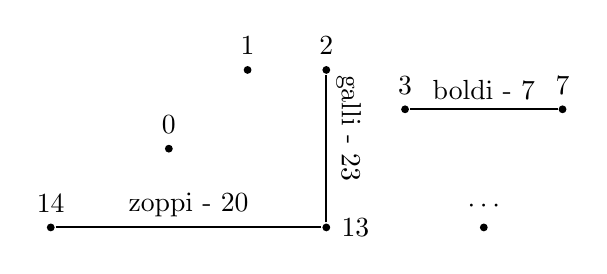
\begin{tikzpicture}
			\node [circle,fill,label=above:{0},inner sep=1pt](0) at (0,0) {};
			\node [circle,fill,label=above:{1},inner sep=1pt](1) at (1,1) {};
			\node [circle,fill,label=above:{2},inner sep=1pt](2) at (2,1) {};
			\node [circle,fill,label=above:{3},inner sep=1pt](3) at (3,0.5) {};
			\node [circle,fill,label=above:{7},inner sep=1pt](7) at (5,0.5) {};
			\node [circle,fill,label=right:{13},inner sep=1pt](13) at (2,-1) {};
			\node [circle,fill,label=above:{14},inner sep=1pt](14) at (-1.5,-1) {};
			\node [circle,fill,label=above:{$\cdots$},inner sep=1pt](d) at (4,-1) {};

			\draw (14) -- (13) node [midway,above] {zoppi - $20$};
			\draw (13) -- (2) node [midway,above, label={[rotate=-90]above:{galli - $23$}}] {};
			\draw (3) -- (7) node [midway,above] {boldi - $7$};
		\end{tikzpicture}

	\end{center}
	\caption{Grafo associato per la costruzione di una struttura per funzioni statiche.}%
	\label{fig:static_graph}
\end{figure}
Trasformeremo ora il grafo in un sistema di equazioni: ogni vertice è una variabile $w_0, w_1, \cdots, w_{m-1}$ e ad ogni lato corrisponde
l'equazione
$$
	\forall x \in X ~~ (w_{h_1(x)} + w_{h_2(x)}) \mod 2^r = f(x)
$$
Se il grafo è aciclico (che è un'assunzione) il sistema è risolvibile. 
L'esistenza di una sequenza di peeling (che esiste se e solo se il grafo è aciclico) significa 
che si possono ordinare le equazioni in modo che una delle due variabili non sia mai 
comparsa prima: questo significa che la soluzione si può trovare ordinando le equazioni
e assegnando il valore che rende vera l'equazione alla variabile che non è ancora apparsa. 
Quindi, per esempio
$$
\begin{cases}
    (w_{14} + w_{13}) \mod 2^5 = 20 \\
    (w_{2} + w_{13}) \mod 2^5 = 23 \\
    (w_{3} + w_{7}) \mod 2^5 = 7 \\
\end{cases}
$$
Usando come hinge $w_{14} = 20$, $w_{2} = 23$ e $w_{7} = 7$ si risolve il sistema. 

\subsubsection{Implementazione}
Una volta memorizzate le soluzioni $w_i$ del sistema in un vettore $\mathbf{w}$, 
si può calcolare $f(x)$ per ogni $x \in X$ come 
$$
f(x) = (w_{h_1(x)} + w_{h_2(x)}) \mod 2^m 
$$
Bisogna però decidere la grandezza di $m$, ossia il numero di vertici (o il numero di bucket, o il numero 
massimo che può risultare da un hash): è facile vedere che se $m$ è ``troppo piccolo'' è molto imporbabile 
che riescano a soddisfare le condizioni, ossia si troveranno cicli, collisioni e così via. Se si 
sceglie ``troppo grande'', la struttura che si memorizza occupa molto spazio. 
Precisamente, questo tradeoff dipende da quanto è probabile che il grafo generato sia aciclico. 
\begin{theorem}
    Se $m > (2.09 \cdot |X|)$, il grafo è ``quasi sempre'' aciclico. Il numero atteso di tentativi 
    di generazione di coppie di funzioni hash è circa $2$.
\end{theorem}
\begin{proof}
    Omessa.
\end{proof}

Naturalmente si può anche calcolare la funzione di un qualcosa che non è tra gli input desiderati e 
qualcosa verrà prodotto, ma non avrà un senso ben inteso. 

\subsubsection{Spazio}
Il vettore che dobbiamo memorizzare ha $m$ elementi, ognuno dei quali contiene $r$ bit: in tutto, 
il vettore occupa spazio $m\cdot r$ bit. Definendo $|X| = n$, dal teorema precedente si ha 
$m\cdot r \geq 2.09nr$; lo spazio totale si trova aggiungendo lo spazio per memorizzare 
le funzioni di hash $h_1$ e $h_2$.  

Tutto questo processo può essere eseguito non solo per i grafi (costruiti con $2$ funzioni hash)
ma anche per gli ipergrafi, costruendo un $r$-ipergrafo utilizzando $r$ funzioni hash. Ci si può 
quindi chiedere quale sia la costante che rende ipergrafi con $r > 2$ ``quasi sempre'' aciclici: 
\begin{theorem}
    Per ogni $k$-ipergrafo esiste una costante $\gamma_k$ tale che se $m > \gamma_k n$ allora 
    l'ipergrafo ammette quasi sempre una sequenza di peeling. 
\end{theorem}
\begin{proof}
    Omessa.
\end{proof}

In effetti, le costanti $\gamma_k$ hanno un minimo in $k = 3$: il meglio che si può 
ottenere è quindi utilizzando $3$ funzioni di hash. Il numero di bit che consuma 
$\mathbf{w}$ è quindi $1.23nr$ bit.  

\begin{table}[htpb]
    \centering
    \begin{tabular}{c|c}
	 $k$ &  $\gamma_k$ \\ 
	 \hline 
	 2 & 2.09 \\
	 3 & 1.23 \\
	 $\cdots$ & > 1.23 $\cdots$
    \end{tabular}
    \caption{Costanti $\gamma_k$ per $k$-ipergrafi.}
    \label{tab:gamma_k_hypergraph}
\end{table}

\subsubsection{Lower bound}
Per capire che tipo di struttura stiamo costruendo, dobbiamo calcolare l'information-theoretical 
lower bound. Stiamo memorizzando una funzione da un insieme $X$ fissato ad un insieme $2^r$.  
Le funzioni di questo tipo sono ${2^{r}}^{|X|} = 2^{r|X|} = 2^{rn}$, definendo come prima $|X| = n$. 
Quindi, l'information-theoretical lower bound è 
$$
Z_n = \log_2(2^{rn}) = rn \text{ bit}
$$
e la struttura che abbiamo descritto occupa 
$$
D_n = 1.23nr = O(Z_n) \text{ bit}
$$
pertanto la struttura è compatta.

\subsubsection{Struttura compressa}
Si può osservare che nel vettore $\mathbf{w}$ molte entry sono uguali a $0$: il numero 
di entry diverse da zero è pari al numero di hinge nella sequenza di peeling 
che risolve il sistema generato dal grafo, quindi $\mathbf{w}$ che (assumendo 
l'utlizzo di $3$ funzioni di hash) ha esattamente $m = 1.23n$ elementi, al più
$n$ elementi sono non nulli. 

Quindi, si possono memorizzare unicamente gli elementi non nulli in $\tilde{\mathbf{w}}$ 
utilizzando un ulteriore array $\mathbf{b}$ di $m$ bit tale che 
$$
\mathbf{b}[i] = \begin{cases}
    1 & \mathbf{w}[i] \neq 0 \\
    0 & \mathbf{w}[i] = 0
\end{cases}
$$
definendo quindi il vettore 
$$
\mathbf{w}[i] = \begin{cases}
    0 & \mathbf{b}[i] = 0 \\
    \tilde{\mathbf{w}}[\mathbf{rank_b}[i]] & \mathbf{b}[i] = 1
\end{cases}
$$
In questo modo, la struttura (che è comunque compatta) in totale occupa 
$$
D_n = nr + m = nr + 1.23n = (r + 1.23) n \text{ bit}
$$
e si ha quindi 
$$
(r + 1.23 ) n < 1.23rn \implies (r + 1.23) < 1.23r  \implies r > 5
$$

\noindent
Inizialmente, la tecnica MWHC era stata pensata per un uso ben più specifico, 
ossia memorizzare una funziona di hash minimale perfetta, ossia una funzione
che mappa $n$ chiavi in $n$ bucket privi di collisioni. 
Tuttavia questa tecnica è abbastanza generale da memorizzare qualsiasi funzione e 
si può utilizzare questa tecnica come intesa inizialmente semplicemente associando 
$f(x)$ diversi da $0$ a $n-1$ per ogni elemento di $X$. 
